%%%%%%%%%%%%%%%%%%%%%%%%%%%%%%%%%%%%%%%%%%%%%%%%%%%%%%%%%%%%%%%%%%%%%%%%%
%%%%%%%%%%%%%%%%%%%%%%%%%%%%%%%%%%%%%%%%%%%%%%%%%%%%%%%%%%%%%%%%%%%%%%%%%
%%%% Plantilla realizada por César Martínez cesar.martinez@udlap.mx %%%%%
%%%%%%%%%%%%%%%%%%%%%%%%%%%%VERSION 1.0%%%%%%%%%%%%%%%%%%%%%%%%%%%%%%%%%%
%%%%%%%%%%%%%%%%%%%%%%%%%%%%%%%%%%%%%%%%%%%%%%%%%%%%%%%%%%%%%%%%%%%%%%%%%
%%%%%%%%%%%%%%%%%%%%%%%%%%%%%%%%%%%%%%%%%%%%%%%%%%%%%%%%%%%%%%%%%%%%%%%%%


\documentclass[12pt]{article}  %tipo de documento y tamaño de letra normal
%%%%%%%%%%%%%%%%%%%%%%%%%%%%%%%%%%%%%%%%%%%%%%%%%%%%%%%%%%%%%%%%%%%%%
%%%%%%%%%%%%%%%%%%%%%%%%%%%%%%%%%%%%%%%%%%%%%%%%%%%%%%%%%%%%%%%%%%%%%
%%%%%%%%%%%%%%%%%%%%%%%%%%%%%%%%%%%%%%%%%%%%%%%%%%%%%%%%%%%%%%%%%%%%%
%%%%%%%% Paquetes basicos, pueden encontrar información especifica de cada uno de ellos en  (https://www.ctan.org/) %%%%%%%%%%%%%%%%%%%%%%% %%%%%%%%%%%%%%%%%%%%%%%%%%%%%%%%%%%%%%%%%%%%%%%%%%%%%%%%%%%%%%%%%%%%%
%%%%%%%%%%%%%%%%%%%%%%%%%%%%%%%%%%%%%%%%%%%%%%%%%%%%%%%%%%%%%%%%%%%%%
%%%%%%%%%%%%%%%%%%%%%%%%%%%%%%%%%%%%%%%%%%%%%%%%%%%%%%%%%%%%%%%%%%%%%
%\usepackage[spanish]{babel} %Indica que escribiermos en español
\usepackage[english]{babel} %Indica que escribiermos en inglés
%Comentar la línea del idioma que NO usarán en su reporte
\usepackage[utf8]{inputenc} %Indica qué codificación se está usando ISO-8859-1(latin1)  o utf8
\usepackage{amsmath} % Comandos extras para matemáticas (cajas para ecuaciones,etc)
\usepackage{amssymb} % Simbolos matematicos (por lo tanto)
\usepackage{graphicx} % Incluir imágenes en LaTeX
\usepackage{color} % Para colorear texto
\usepackage{subfigure} % subfiguras
\usepackage{enumerate} % enumerar
\usepackage{commath} % funcionalidades extras para diferenciales, integrales,etc (\od, \dif, etc)
\usepackage{cancel} % para cancelar expresiones (\cancelto{0}{x})
\usepackage{float} %Podemos usar el especificador [H] en las figuras para que se queden donde queramos
\usepackage{appendix} %Para crear apendices
\usepackage{xcolor} %Definir colores personalizados
%%%%%%%%%%%%%%%%%%%%%%%%%%%%%%%%%%%%%%%%%%%%%%%%%%%%%%%%%%%%%%%%%%%%%
%%%%%%%%% PAQUETES CON OPCIONES ESPECIFICAS PRECARGADAS %%%%%%%%%%%%%
%%%%%%%%%%%%%%%%%%%%%%%%%%%%%%%%%%%%%%%%%%%%%%%%%%%%%%%%%%%%%%%%%%%%%
%%%%%%%%%%%%% Permitir agregar código, colocarlo en un rectángulo y  numerarlo %%%%%%%%%%%%%%%%%%%%%%%%%%%%%%%%%%%%%%%%%%%%%%%%%%%%%%%%%%%
%%%%%%%%%%%%%%%%%%%%%%%%%%%%%%%%%%%%%%%%%%%%%%%%%%%%%%%%%%%%%%%%%%%%%
%%%%%%%%%%%%%%%%%%%%%%%%%%%%%%%%%%%%%%%%%%%%%%%%%%%%%%%%%%%%%%%%%%%%%%%%%%%%%%%%%%%%%%%%%%%%%%%%%%%%%%%%%%%%%%%%%%%%%%%%%%%%%%%%%%%%%%%%%%
\usepackage{listings} %Sirve para pegar codigo fuente de programas
\usepackage{caption} %Agregar titulos a los codigos
\DeclareCaptionFont{white}{\color{white}}
\DeclareCaptionFormat{listing}{%
  \parbox{\textwidth}{\colorbox{gray}{\parbox{\textwidth}{#1#2#3}}\vskip-4pt}}
\captionsetup[lstlisting]{format=listing,labelfont=white,textfont=white}
\lstset{frame=lrb,xleftmargin=\fboxsep,xrightmargin=-\fboxsep}
\renewcommand{\lstlistingname}{Código}
%%%%%%%%%%%%%%%%%%%%%%%%%%%%%%%%%%%%%%%%%%%%%%%%%%%%%%%%%%%%%%%%%%%%%
%%% Definir márgenes del documento%%%%%%%%%%%%%%%%%%%%%%%%%%%%%%%%%%%
%%%%%%%%%%%%%%%%%%%%%%%%%%%%%%%%%%%%%%%%%%%%%%%%%%%%%%%%%%%%%%%%%%%%%
 \usepackage{anysize} % Para personalizar el ancho de  los márgenes
\marginsize{2cm}{2cm}{2cm}{2cm} % Izquierda, derecha, arriba, abajo
%%%%%%%%%%%%%%%%%%%%%%%%%%%%%%%%%%%%%%%%%%%%%%%%%%%%%%%%%%%%%%%%%%%%
%%% Hipervinculos activos y a color %%%%%%%%%%%%%%%%%%%%%%%%%%%%%%%%
%%%%%%%%%%%%%%%%%%%%%%%%%%%%%%%%%%%%%%%%%%%%%%%%%%%%%%%%%%%%%%%%%%%%%
\usepackage[colorlinks=true,plainpages=true,citecolor=blue,linkcolor=black]{hyperref}
\usepackage{hyperref}
%%%%%%%%%%%%%%%%%%%%%%%%%%%%%%%%%%%%%%%%%%%%%%%%%%%%%%%%%%%%%%%%%%%%%
%%%%%% Encabezado y pie de pagina %%%%%%%%%%%%%%%%%%%%%%%%%%%%%%%%%%%
%%%%%%%%%%%%%%%%%%%%%%%%%%%%%%%%%%%%%%%%%%%%%%%%%%%%%%%%%%%%%%%%%%%%%
\usepackage{fancyhdr}
\pagestyle{fancy}
\fancyhf{}
\fancyhead[L]{\footnotesize UDLAP} %encabezado izquierda
\fancyhead[R]{\footnotesize CEM}   % encabezado derecha
\fancyfoot[R]{\footnotesize \curso}  % Pie derecha
\fancyfoot[C]{\thepage}  % centro
\fancyfoot[L]{}  %izquierda
\renewcommand{\footrulewidth}{0.4pt}
%%%%%%%%%%%%%%%%%%%%%%%%%%%%%%%%%%%%%%%%%%%%%%%%%%%%%%%%%%%%%%%%%%%%%
%%%% Carpeta donde se deben colocar las imagenes %%%%%%%%%%%%%%%%%%%%
\graphicspath{{Imagenes/}} %Colocar aqui todas las imagenes del documento pueden estar en formato png, eps o jpg, se recomienda eps para mayor calidad.
%%%%%%%%%%%%%%%%%%%%%%%%%%%%%%%%%%%%%%%%%%%%%%%%%%%%%%%%%%%%%%%%%%%%%
%%%%%%%%%%%%%%%%%%%%%%%%%%%%%%%%%%%%%%%%%%%%%%%%%%%%%%%%%%%%%%%%%%%%%
%%%%%%%% Termina carga de paquetes %%%%%%%%%%%%%%%%%%%%%%%%%%%%%%%%%%%
%%%%%%%%%%%%%%%%%%%%%%%%%%%%%%%%%%%%%%%%%%%%%%%%%%%%%%%%%%%%%%%%%%%%%
%%%%%%%%%%%%%%%%%%%%%%%%%%%%%%%%%%%%%%%%%%%%%%%%%%%%%%%%%%%%%%%%%%%%%
%%%%%%%%%%%%%%%%%%%%%%%%%%%%%%%%%%%%%%%%%%%%%%%%%%%%%%%%%%%%%%%%%%%%%
%%%%%% Modificar campos que aparecerán en portada %%%%%%%%%%%%%%%%%%%
%%%%%%%%%%%%%%%%%%%%%%%%%%%%%%%%%%%%%%%%%%%%%%%%%%%%%%%%%%%%%%%%%%%%%
%%%%%%%%%%%%%%%%%%%%%%%%%%%%%%%%%%%%%%%%%%%%%%%%%%%%%%%%%%%%%%%%%%%%%
%%%%%%%%%%%%%%%%%%%%%%%%%%%%%%%%%%%%%%%%%%%%%%%%%%%%%%%%%%%%%%%%%%%%%
\def\titulo{Reporte de laboratorio \#6}%titulo del documento
\def\materia{Curso: Diseño digital LRT2022-1} %Clave nombre de la materia y sección
\def\curso{Diseño Digital} %Nombre de la materia para footnote
\def\fecha{14 de Noviembre del 2023} %En formato mes, dia año
\def\equipo {Mesa 1}%Verificar en blackboard el número asignado
\def\ida{ID: 178432} %Nombre y Id´s de todos los integrantes que hayan trabajado en el proyecto
\def\esta{Fernanda Sofía Ovalle Prado}
\def\lica{LBM}%LRT,LBM,LIS,LMT
\def\idb{177516} %Nombre y Id´s de todos los integrantes que hayan trabajado en el proyecto
\def\estb{Jesus Alvarez Sombrerero}
\def\licb{LIS}%LRT,LBM,LIS,LMT
\def\topic{Circuitos lógicos combinacionales básicos}
%Copiar y pegar más líneas si su equipo tiene más de 5 integrantes, eliminar si está formado por menos
%%%%%%%%%%%%%%%%%%%%%%%%%%%%%%%%%%%%%%%%%%%%%%%%%%%%%%%%%%%%%%%%%%%%%
%%%%%%%%%%%%%%%%%%%%%%%%%%%%%%%%%%%%%%%%%%%%%%%%%%%%%%%%%%%%%%%%%%%%%
%%%%%%%%%%%%%%%%%%%%%%%%%%%%%%%%%%%%%%%%%%%%%%%%%%%%%%%%%%%%%%%%%%%%%
\begin{document} %Inicia el documento
%%%%%%%%%%%%%%%%%%%%%%%%%%%%%%%%%%%%%%%%%%%%%%%%%%%%%%%%%%%%%%%%%%%%%
%%%%%%%%%%%%%%%%%%%%%%%%%%%%%%%%%%%%%%%%%%%%%%%%%%%%%%%%%%%%%%%%%%%%%
%%%%%%%%%%%%%%%%%%%%%%%%%%%%%%%%%%%%%%%%%%%%%%%%%%%%%%%%%%%%%%%%%%%%%
%%%%%%%%%%%%%%%%%%%%%%%%%%%%%%%%%% PORTADA %%%%%%%%%%%%%%%%%%%%%%%%%%
%%%%%%%%%%%%%%%%%%%%%%%%%%%%%%%%%%%%%%%%%%%%%%%%%%%%%%%%%%%%%%%%%%%%%No es necesario modificar ninguna de las siguientes lineas, sólo si el número de estudiantes que conforman su equipo es menor o mayor a 5
%%%%%%%%%%%%%%%%%%%%%%%%%%%%%%%%%%%%%%%%%%%%%%%%%%%%%%%%%%%%%%%%%%%%%
%%%%%%%%%%%%%%%%%%%%%%%%%%%%%%%%%%%%%%%%%%%%%%%%%%%%%%%%%%%%%%%%%%%%%
%%%%%%%%%%%%%%%%%%%%%%%%%%%%%%%%%%%%%%%%%%%%%%%%%%%%%%%%%%%%%%%%%%%%%
\begin{center}
    \newcommand{\HRule}{\rule{\linewidth}{0.5mm}}
    \thispagestyle{empty}
    \vspace*{-1.5cm}
    \textsc{\huge Universidad de las Américas Puebla}\\[1.5cm]
    \textsc{\LARGE Escuela de ingeniería}\\[1.5cm]
    \textsc{\LARGE Departamento de computación, electrónica y mecatrónica}\\[1.5cm]
    \includegraphics[width=150mm]{UDLAP}  									\vspace*{1cm}														\HRule \\[0.4cm]
    { \huge \bfseries \titulo}\\[0.4cm]
    \HRule \\[1cm]
    { \Large \bfseries \materia}\\[1cm]
    { \Large \bfseries Tema: \topic}\\[1cm]
    { \Large \bfseries Equipo: \equipo}\\[1cm]
    \begin{flushleft} \Large
        \ida \hspace{0.5cm}\esta \hspace{0.5cm} \lica\\
        \idb \hspace{0.5cm}\estb \hspace{0.5cm} \licb\\
        %Copiar y pegar más líneas si su equipo tiene más de 2 integrantes, eliminar si la entrega es individual
    \end{flushleft}
    \vfill
    \begin{center}
        {\Large  \fecha, San Andrés Cholula, Puebla}
    \end{center}
\end{center}							 								\newpage
%%%%%%%%%%%%%%%%%%%% TERMINA PORTADA %%%%%%%%%%%%%%%%%%%%%%%%%%%%%%%%
%%%%%%%%%%%%%%%%%%%%%%%%%%%%%%%%%%%%%%%%%%%%%%%%%%%%%%%%%%%%%%%%%%%%%
%%%%%%%%%%%%%%%%%%%%%%%%%%%%%%%%%%%%%%%%%%%%%%%%%%%%%%%%%%%%%%%%%%%%%
%%%%%%%%%%%%%%%%%%%%%%%%%%%%%%%%%%%%%%%%%%%%%%%%%%%%%%%%%%%%%%%%%%%%%
%%%%%%%%%%%%%%%%%%%%%%%%%%%%%%%%%%%%%%%%%%%%%%%%%%%%%%%%%%%%%%%%%%%%%
\setcounter{page}{1} %Para comenzar a numerar las páginas desde este punto
\begin{abstract}
En esta práctica programamos un Basys 3 en modo JTAG - USB con códigos escritos en VHDL, programando en asignación de señales concurrentes con operadores lógicos. Hicimos tablas y diagramas para analizar y conseguir las funciones. Comprobamos el funcionamiento de un multiplexor, medio restador, comparador de magnitud y demultiplexor. Concluimos que se comporta igual en el sistema físico de Basys 3, utilizando un testbench y los códigos de VHDL y generando un EPWave con EDA Playground para comprobar que se parecieran a las tablas propuestas para cada circuito combinacional.

\vspace{0.5cm}

\textit{Keywords: Circuitos combinacionales, VHDL, Basys 3, funciones booleanas.}
\end{abstract}

\section*{Objetivos}

\begin{enumerate}
  \item Programar y simmular un circuito básico lógico combinacional en VHDL.
  \item Implementar los circuitos combinacionales básicos en la placa Basys 3.
\end{enumerate}

\section*{Materiales}

\subsection*{Equipamiento}

\begin{itemize}
    \item Basys 3 board
\end{itemize}

\subsection*{Software}

\begin{itemize}
    \item Vivado 2018.2
    \item EDA Playground
\end{itemize}

\section*{Introducción y Marco Teórico}
La Basys 3 es una placa de desarrollo FPGA de nivel básico diseñada exclusivamente para el Vivado Design Suite con la arquitectura AMD Artix 7 FPGA. La FPGA tiene 33,280 celdas lógicas en 5200 rebanadas, cada una con cuatro LUT de 6 entradas y 8 flip-flops. También tiene cinco tiles de gestión de reloj, cada uno con un bucle de fase bloqueada (PLL). La placa tiene un puerto USB-JTAG de Digilent para la programación y comunicación de la FPGA. Este puerto permite cargar el diseño del usuario en la FPGA y depurar el funcionamiento del circuito \cite{Digilent2023}.

Vivado es un entorno de diseño integrado (IDE) desarrollado por Xilinx para el diseño y desarrollo de FPGA. Proporciona una variedad de herramientas para la gestión de IP, diseño lógico, síntesis, implementación y depuración \cite{AMDVivado2023}.

Se puede programar un Basys 3 de tres formas diferentes \cite{Digilent2023Guide}:
\begin{itemize}
  \item JTAG: Esta forma usa el puerto micro-USB para comunicarse con el Basys 3 y enviarle el archivo .bit que contiene el diseño del circuito. Necesitas tener el jumper JP1 en la posición JTAG y usar Vivado para programar el dispositivo.
  \item Quad SPI Flash: Esta forma usa la memoria flash integrada en el Basys 3 para almacenar el archivo .bin que contiene el diseño del circuito. De esta manera, el Basys 3 se programa automáticamente cada vez que se enciende. Necesitas tener el jumper JP1 en la posición QSPI y usar Vivado para escribir el archivo .bin en la memoria flash.
  \item USB Flash Drive: Esta forma usa una memoria USB externa para guardar el archivo .bit que contiene el diseño del circuito. El Basys 3 lee el archivo .bit desde la memoria USB y lo carga en el FPGA cada vez que se enciende. Necesitas tener el jumper JP1 en la posición USB y copiar el archivo .bit en la raíz de la memoria USB.
\end{itemize}

\section*{Analisis Teórico}

\subsection*{Medio Restador}

Un medio restador es un circuito combinacional que puede realizar la operación de sustracción de dos bits. Específicamente, toma dos bits como entrada y produce dos bits de salida: una salida de diferencia y una salida de acarreo \cite{9622531}.

La tabla a la que concluimos que representa es la siguiente, la cual recibe dos bits que son restados de A - B. Se obtiene la diferencia y el acarreo que hay en la operación.

\begin{table}[!ht]
    \centering
    \caption{Medio Restador}
    \begin{tabular}{|l|l|l|l|}
    \hline
        A & B & D(Diferencia) & A (Acarreo) \\ \hline
        0 & 0 & 0 & 0 \\ \hline
        0 & 1 & 1 & 1 \\ \hline
        1 & 0 & 1 & 0 \\ \hline
        1 & 1 & 0 & 0 \\ \hline
    \end{tabular}
\end{table}

En cuanto a su diagrama, se puede simular la salida de la diferencia con un XOR y para mostrar el acarreo, se utiliza un not(A) y un (not(A))and(B). Este se puede analizar de forma sencilla ya que a primera vista se entiende que la diferencia representa una compuerta lógica XOR. A partir de ahí, buscamos la forma de conseguir el acarreo y comprobamos nuestros resultados a mano con la tabla.

\begin{figure}[!ht]
    \centering
    \caption{Diagrama medio restador}
    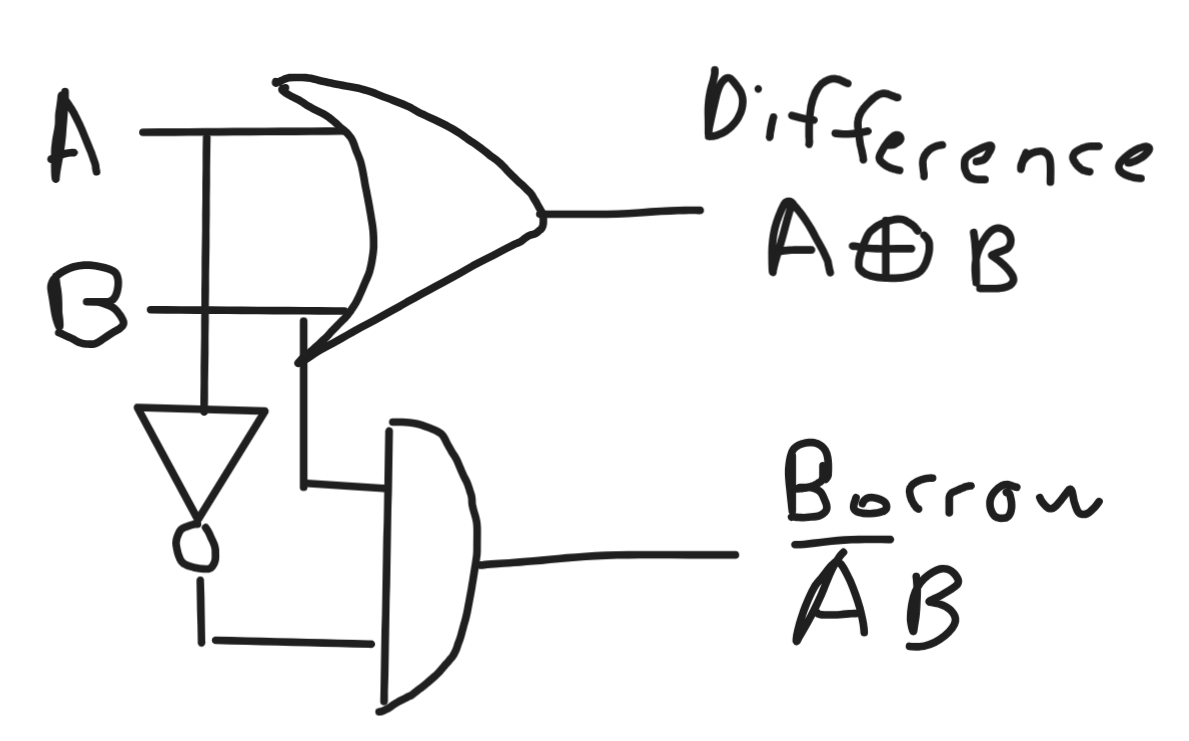
\includegraphics[width=0.25\linewidth]{Imagenes/Schemes/medio-restador.png}
\end{figure}
\newpage

\subsection*{Multiplexor}
Es un circuito combinacional que selecciona una de las muchas entradas y la dirige a una única salida \cite{7944062}.

La tabla del multiplexor es la siguiente, la cual recibe dos inputs, I0 e I1, cuando S es 0, se selecciona el input I0 y cuando S está en 1, se registra I1 como el output O.

\begin{table}[!ht]
    \centering
    \caption{Multiplexor}
    \begin{tabular}{|l|l|l|l|}
    \hline
        S & I0 & I1 & O \\ \hline
        0 & 0 & 0 & 0 \\ \hline
        0 & 0 & 1 & 0 \\ \hline
        0 & 1 & 0 & 1 \\ \hline
        0 & 1 & 1 & 1 \\ \hline
        1 & 0 & 0 & 0 \\ \hline
        1 & 0 & 1 & 1 \\ \hline
        1 & 1 & 0 & 0 \\ \hline
        1 & 1 & 1 & 1 \\ \hline
    \end{tabular}
\end{table}

Otra forma de verlo es con el diagrama, el multiplexor selecciona el input que debe salir en el output dependiendo de su estado.

\begin{figure}[!ht]
    \centering
    \caption{Diagrama multiplexor}
    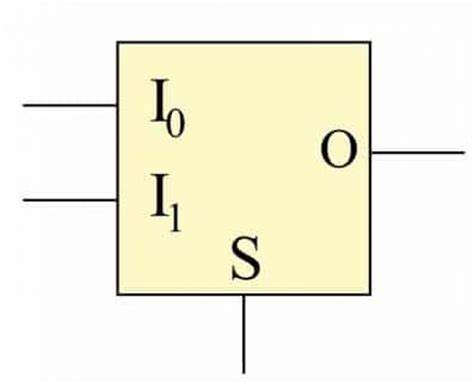
\includegraphics[width=0.25\linewidth]{Imagenes/Schemes/multiplexor.jpg}
\end{figure}

\subsection*{Comparador de magnitud}

Un comparador de magnitud es un circuito combinacional que compara dos números binarios, para averiguar si estos números binarios son iguales, o cual es el número menor y cual es el mayor. El diseño de este circuito se tienen dos entradas, una llamada A y otra llamada B, estos serían los números a comparar. Además tiene tres terminales de salida, una para la condición A mayor que B, otra para la condición A igual a B y la última para la condición A menor que B \cite{ComparadorDeMagnitud}. 

La tabla de verdad de un comparador de magnitud de un bit es la siguiente:
\begin{table}[!ht]
	\centering
        \caption {Tabla de verdad del comparador de magnitud}
	\begin{tabular}{|l|l|l|l|l|}
	\hline
	    A	&  B  & A < B  & A = B  & A > B  \\\hline 
         0  &  0  &  0  &  1  &  0 \\ \hline 
         0  &  1  &  1  &  0  &  0 \\  \hline 
         1  &  0  &  0  &  0  &  1 \\ \hline 
         1  &  1  &  0  &  1  &  0 \\ \hline
 \end{tabular}
 \end{table}
 
\subsection*{Demultiplexor}

El demultiplexor se utiliza para enviar señales a los dispositivos. Este consta de una entrada con diferentes líneas de salida. El demultiplexor toma una señal y las codifica en diferentes cables, osea hace todo lo contrario a lo que hace un multiplexor \cite{Electricidad}.

La tabla de verdad de un demultiplexor de un bit es la siguiente:

\begin{table}[!ht]
	\centering
	\begin{tabular}{|l|l|l|l|}
\hline Entrada (A) & Canal de selección (S) & Salida 1 (Y0) & Salida 2 (Y1)  \\
\hline 0 & 0 & 0 & 0 \\ 
\hline 0 & 1 & 0 & 0 \\ 
\hline 1 & 0 & 0 & 1 \\ 
\hline 1  &  1  & 1 & 0 \\  

   \hline
	\end{tabular}
	\caption {Tabla de verdad del demultiplexor}
	\label{Tabla:1}
 \end{table}
 
\section*{Registros}
Lo que concluimos es que a pesar de que se puede representar con una función booleana los circuitos combinacionales, es posible abstraerlos a un método de selección. El método de programación que escogimos es asignación concurrente. En cuanto a los testbench y las EPWaves, se utilizó EDA Playground para comprobar sus funcionamientos.

\subsection*{Códigos y EPWaves}

\subsubsection*{Medio Restador}

El siguiente es el código de el medio restador. Utilizando los diagramas del medio restador que utilizamos para comprobar la tabla, codificamos una función Difference y una Borrow. Difference representar el XOR y Borrow representa el not y and que salen en el diagrama. Se obtienen dos resultados y para ello se deben realizar dos outputs en el testbench.

\lstinputlisting[language=VHDL,caption=Código medio restador]{codigos/combinational/half.vhd}

El testbench del medio restador tiene los outputs Difference y Borrow asignados como se mencionó. Hay que aclarar que EDA Playground, que es el simulador que utilizamos, no permite una entidad que no sea testbench en el archivo que va a hacer de testbench y es por eso que cambiamos el nombre al correspondiente. De ahí solo mandamos 4 señales debido a que solo hay 2 inputs y 2 al cuadrado son 4 (Testbench completo en anexos).

\lstinputlisting[language=VHDL,caption=Código Testbench medio restador,firstline=1, lastline=15]{codigos/tests/halftest.vhd}

La EPWave del medio restador es la siguiente, la cual sale duplicada pero demuestra correctamente los resultados del test en 100,000ps. Por ejemplo, podemos ver el comportamiento del XOR en el Difference y el único 1 que sale en el Borrow que es cuando B está activo y A está apagado ya que A se debe negar para que se active el Borrow.

\begin{figure}[!ht]
    \centering
    \caption{EPWave medio restador}
    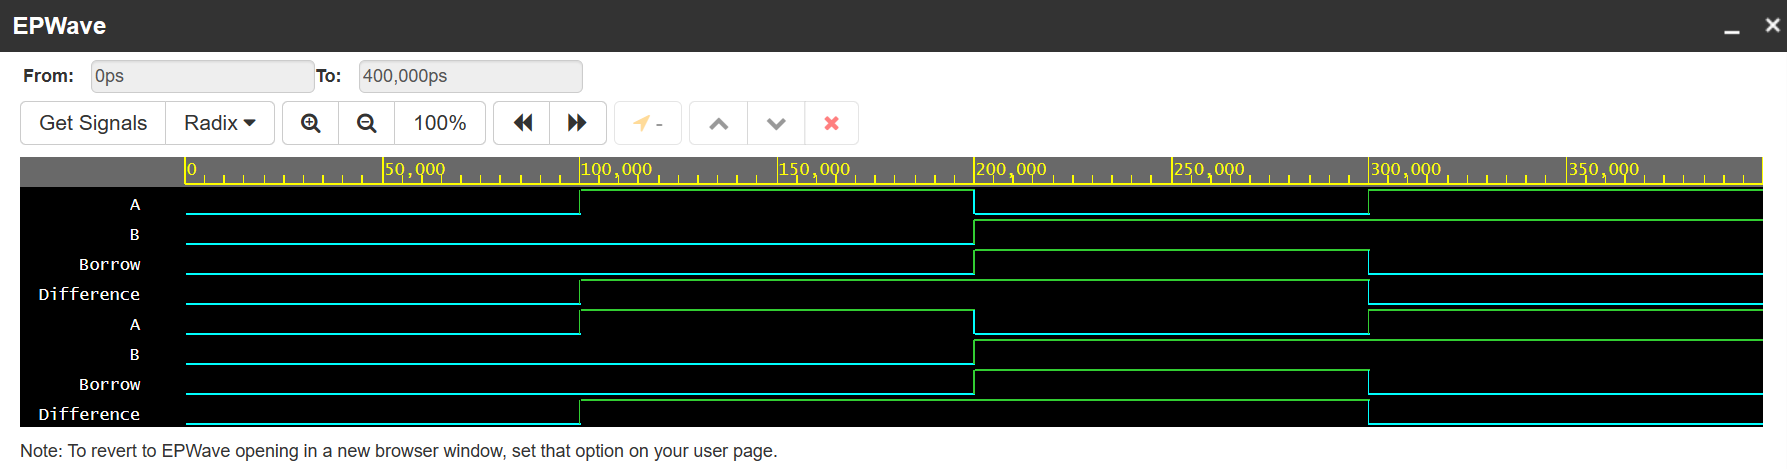
\includegraphics[width=0.8\linewidth]{Imagenes/waves/halfwave.png}
\end{figure}

\subsubsection*{Multiplexor}
(A and not S) or (B and S);
Para el multiplexor analizamos lo que más nos convenía para obtener una función que satisfazca la tabla. Si lo consideramos como 3 inputs en vez de 2 inputs y 1 selector, podemos activar a A cuando S no está activada y activar a B cuando S está encendida. A y B representan a I0 e I1 respectivamente. Así, por ejemplo, cuando B sea 1, y S sea 1, se cumple la condición del AND en la siguiente función: Y(ABS) = (A and not S) or (B and S), donde Y representa O, el output, y A y B son I0 e I1. De igual forma si S sigue siendo 1 pero B es 0, tendremos de todas formas la representación de los inputs de B.

\lstinputlisting[language=VHDL,caption=Código multiplexor]{codigos/combinational/multiplexer.vhd}

El testbench tuvimos que separar un poco la lógica de forma visual para que se entienda. Tenemos dos pruebas en una sola, una para cada estado de S, aunque bien se pueden considerar para el mismo S, simplemente quisimos separar un poco los casos para representar mejor al multiplexor como un circuito combinacional de selección. De ahí en fuera, se mantiene la entidad testbench y se maneja igual el nombre de inputs y outputs, aunque en este caso son 3 inputs y 3 outputs ya que aunque el multiplexor igual se puede considerar como un selector, fuera de la abstracción es un input (Testbench completo en anexos).

\lstinputlisting[language=VHDL,caption=Código Testbench multiplexor,firstline=1, lastline=15]{codigos/tests/multiplexertest.vhd}

La EPWave del multiplexor es el siguiente, que demuestra cómo el estado de A/I0 se refleja en Y cuando S es 0 y el estado de B/I1 se refleja y el estado de S es 1.

\begin{figure}[!ht]
    \centering
    \caption{EPWave multiplexor}
    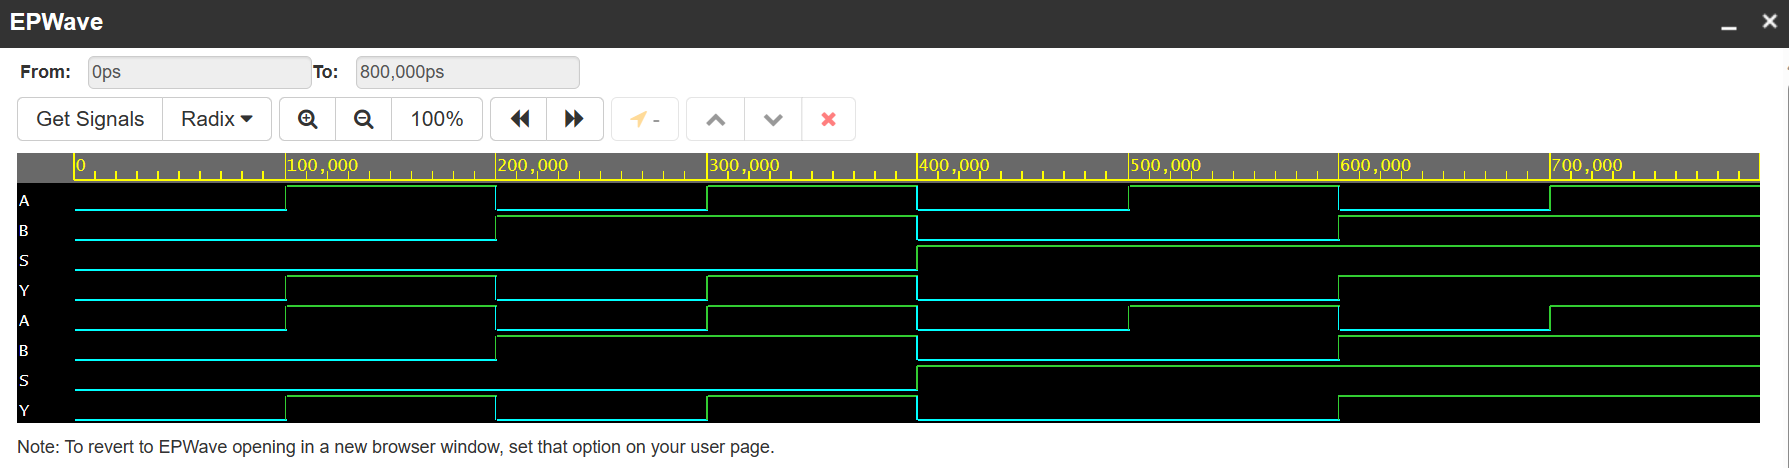
\includegraphics[width=1\linewidth]{Imagenes/waves/multiplexer.png}
\end{figure}

\subsubsection*{Comparador de Magnitud}
El comparador de magnitud decidimos codificarlo en señales condicionales, así que establecimos el nombre para dos entradas, en este caso A sería la entrada a comparar con la entrada B. Luego establecimos tres diferentes salidas, una llamada AeqB, esta salida es la encargada de ver si A y B son iguales. A otra salida la llamamos AltB, esta sería la encargada de checar si A es menor que B. Y la última salida, la llamamos AgtB, esta salida nos indicará cuando A sea mayor que B.

\lstinputlisting[language=VHDL,caption=Código Comparador de magnitud,firstline=1, lastline=15]{codigos/combinational/comparador-mag.vhd}

Para el testbench, seguimos una lógica de modo que hicimos un código para dos entradas (inputs) y tres salidas (outputs). El nombre de las salidas y las entradas se quedaron igual para que no se perdierá el orden. Se codificaron todas las entradas posibles, de modo que A o B fueran 0's y 1's.
\lstinputlisting[language=VHDL,caption=Código Testbench Comparador de magnitud,firstline=1, lastline=15]{codigos/tests/comparador-mag_testbench.vhd}

Con el EPWave que nos da el testbench, podemos ver que nos da los valores las tablas de verdad, se activan las salidas dependiendo de los valores de las entradas.

\begin{figure}[!ht]
    \centering
    \caption{EPWave Comparador de magnitud}
    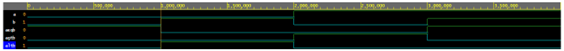
\includegraphics[width=1\linewidth]{Imagenes/waves/comp-mag.png}
\end{figure}

\subsubsection*{Demultiplexor}

Para el demultiplexor usamos la asignación concurrente para la codificación. Seleccionamos una entrada, llamada A, y un canal de selección, llamada S, para los inputs. Para los outputs, como el demultiplexor es de un bit, solo tendremos dos salidas, una llamada Y0 y otra llamada Y1, dentro de estas pusimos las condiciones en las que iban a dar 1 como output.

\lstinputlisting[language=VHDL,caption=Código demultiplexor,firstline=1, lastline=15]{codigos/combinational/demultiplexor.vhd}

Para el testbench diseñamos un código con dos inputs y dos outputs, cada una con el nombre que ya les habíamos dado anteriormente. Decidimos codificar solo el comportamiento de A = 1, ya que si A = 0, todas las salidas serían 0, sin importar el canal de selección.

\lstinputlisting[language=VHDL,caption=Código Testbench demultiplexor,firstline=1, lastline=15]{codigos/tests/demultiplexor_testbench.vhd}

La EPWave del demultiplexor muestra el estado de A y como van cambiando los valores de las salidas, dependiendo S.

\begin{figure}[!ht]
    \centering
    \caption{EPWave demultiplexor}
    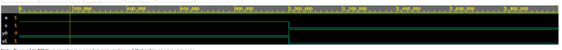
\includegraphics[width=1.1\linewidth]{Imagenes/waves/demux-ep.png}
\end{figure}

\subsection*{Basys 3}
Ya con estos códigos junto con sus testbench hechos, podemos pasar a hacer la implementación física, porque los códigos fueron la simulación del circuito, ya ahora que comprobamos que funcionan los códigos se puede pasar a un hardware. En este caso, usamos un Basys 3 para ver que las condiciones de cada circuito combinacional se cumplía. Vamos a poner ejemplos de las tablas, mientras que las simulaciones completas están en el anexo. Utilizamos el modo JTAG con USB.

\subsubsection*{Medio Restador}
La programación de este circuito combinacional requirió simplemente de activar 2 switches y 2 leds. SW 0 corresponde al A y SW 1 corresponde a B, que son los switches ubicados a la derecha abajo y que van de derecha a izquierda. En cuanto a los leds LD0 y LD1 se utilizan para Difference y Borrow, todo hablando en cuanto al código.

Como ejemplo podemos ver que 0 - 0 da 0.

\begin{figure}[!ht]
    \centering
    \caption{A está en 0 y B está en 0}
    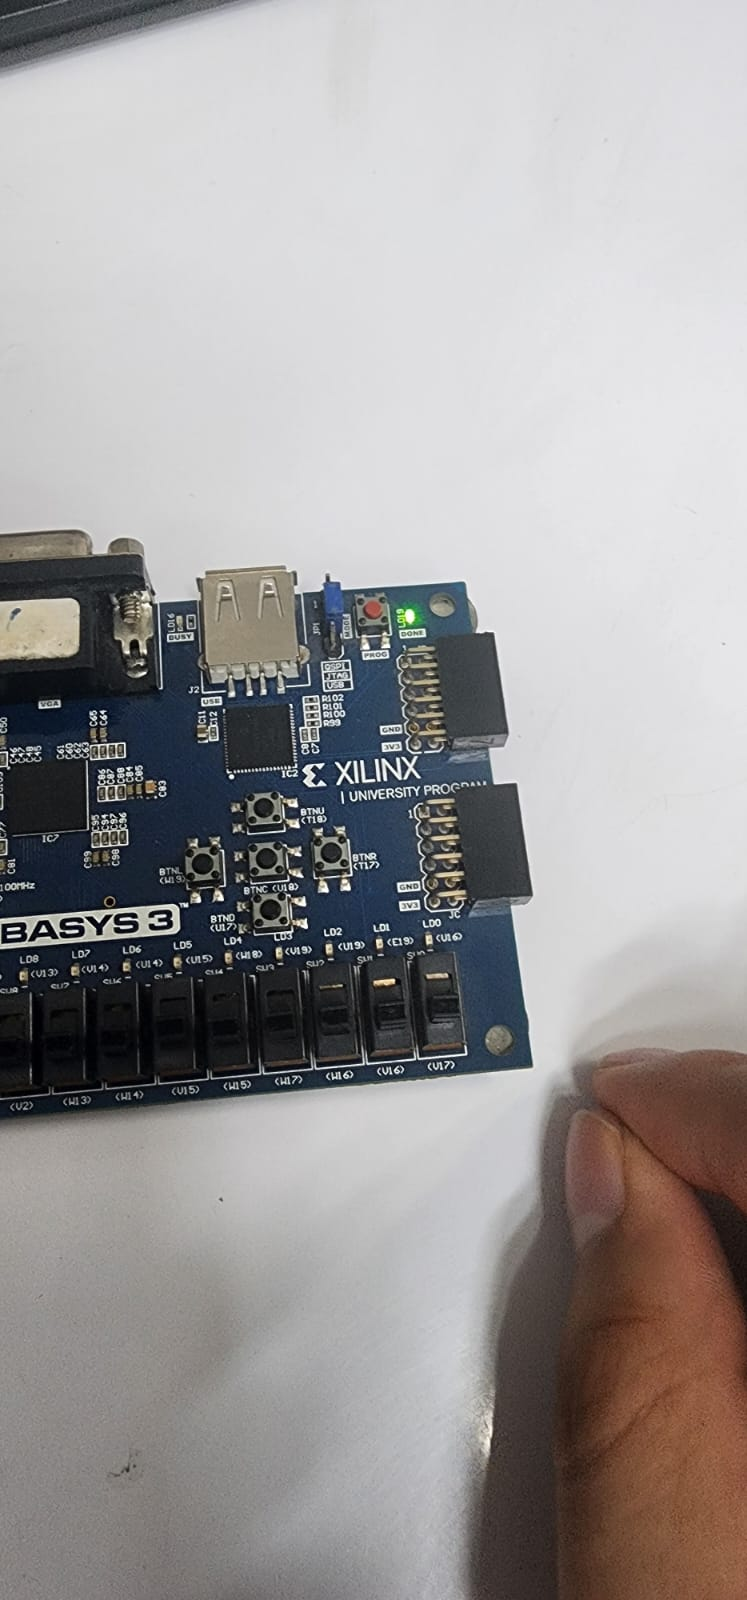
\includegraphics[width=0.4\linewidth]{simulations/half/half0.jpg}
\end{figure}
\newpage

Por otro lado, si restamos 0 - 1, debemos acarrear y tendremos la resta que dará 1.

\begin{figure}[!ht]
    \centering
    \caption{A está en 0 y B está en 1}
    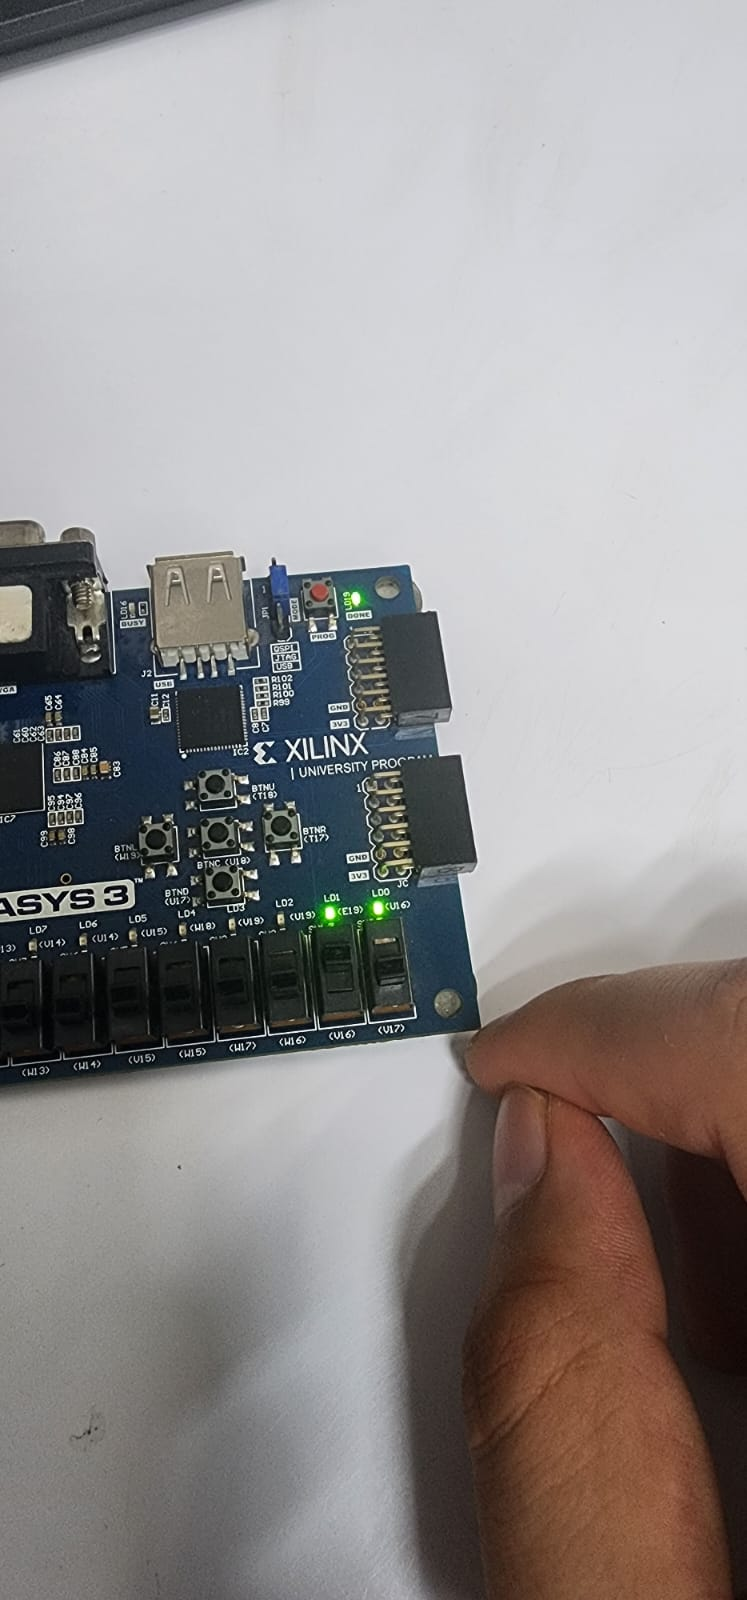
\includegraphics[width=0.4\linewidth]{simulations/half/half2.jpg}
\end{figure}

\subsubsection*{Multiplexor}
En cuanto al multiplexor sucedió que usamos SW0, SW1 y SW2 para A, B y S respectivamente. Se utiliza el código del multiplexor, y así sabemos que Y es la led que intentamos prender LD0. Siguiendo la tabla de del multiplexor, cuando S es 0, y la I0 es 1, donde I0 es el valor correspondiente antes mencionado, tenemos que el output es el mismo I0. Para S es 1, y I1 es su correspondiente en 1, la salida es 1 del I1. Para ambos caso, cuando está seleccionado, no importa el otro.

Por ejemplo, si tenemos el siguiente selector de I0.

\begin{figure}[!ht]
    \centering
    \caption{S está en 0, A está en 1 y B está en 0}
    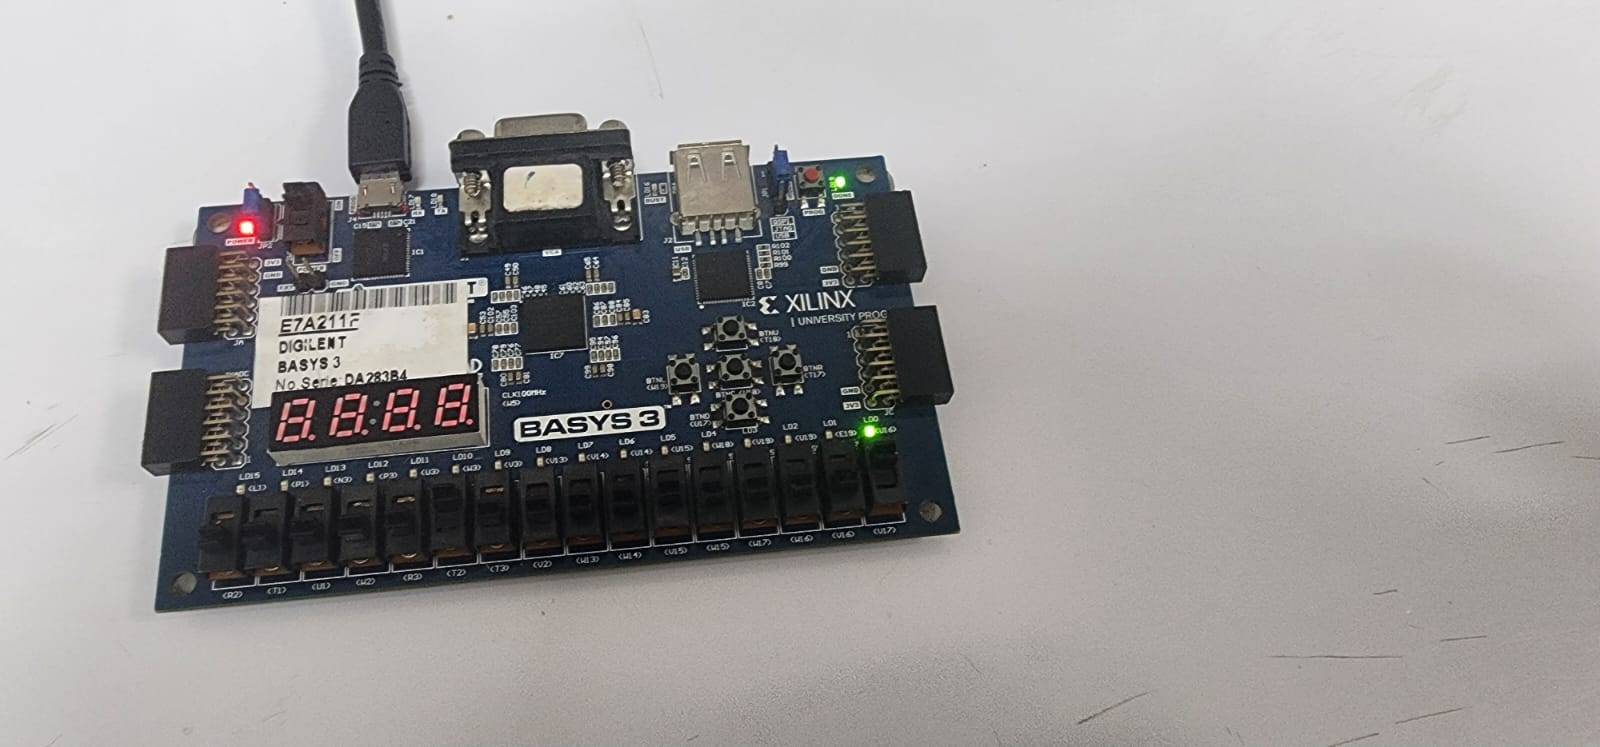
\includegraphics[width=1\linewidth]{simulations/multiplex/multiplex2.jpg}
\end{figure}

Por otro lado cuando seleccionamos a I1.

\begin{figure}[!ht]
    \centering
    \caption{S está en 1, A está en 0 y B está en 1}
    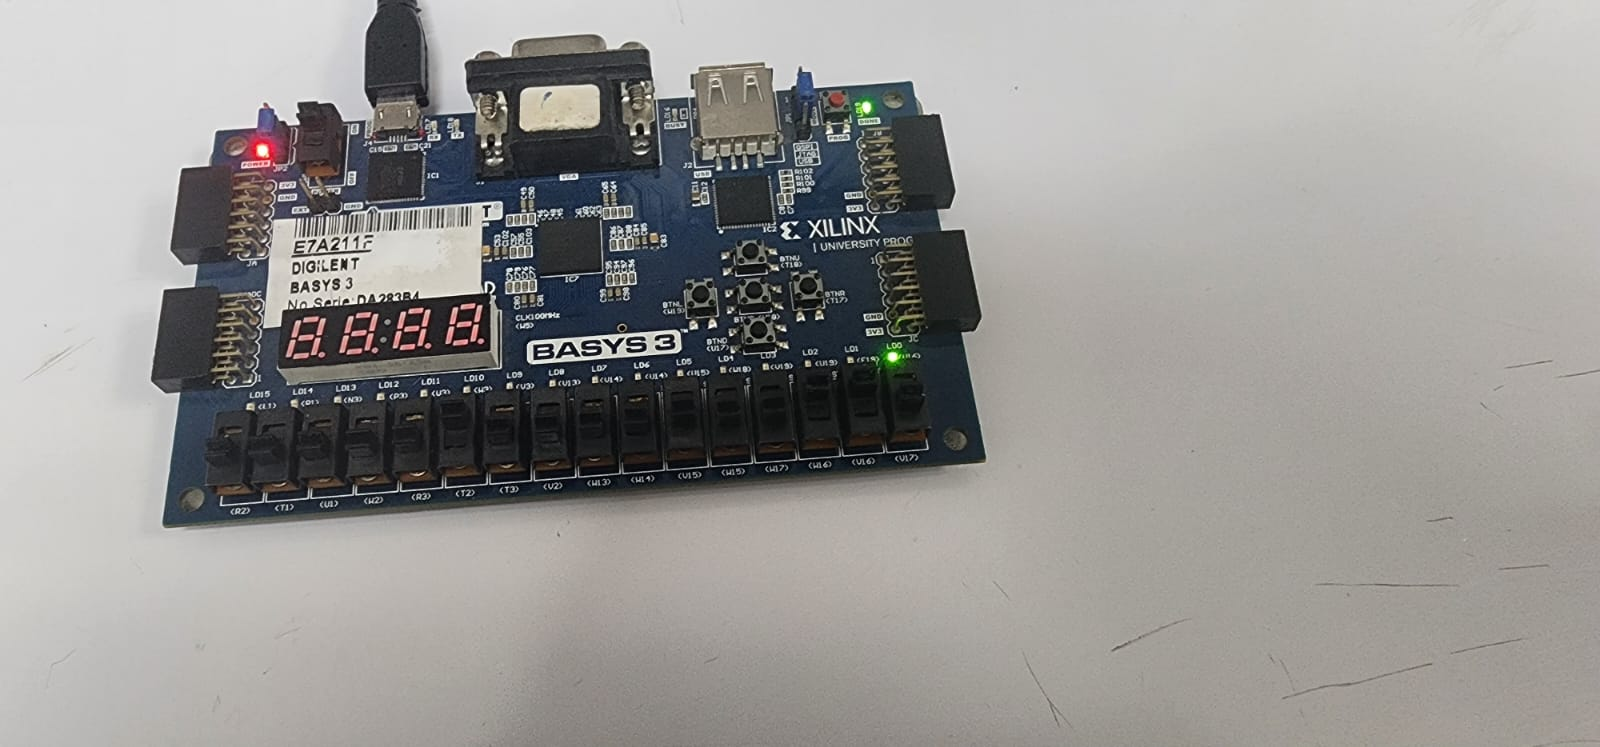
\includegraphics[width=1\linewidth]{simulations/multiplex/multiplex5.jpg}
\end{figure}

\subsubsection*{Comparador de Magnitud}

Como este circuito tiene dos entradas y tres salidas, las entradas que nosotros establecimos en el hardware fueron, switch 0 para B y switch 1 para A. En las salidas, el led 0 sería la AeqB, el led 1 sería AltB, y el led 2 sería AgtB.

En la figura 7, vemos que se está cumpliendo la condición de AgtB ya que está prendido el led 2.
\newpage
\begin{figure}[!ht]
    \centering
    \caption{A está en 1 y  B está en 0}
    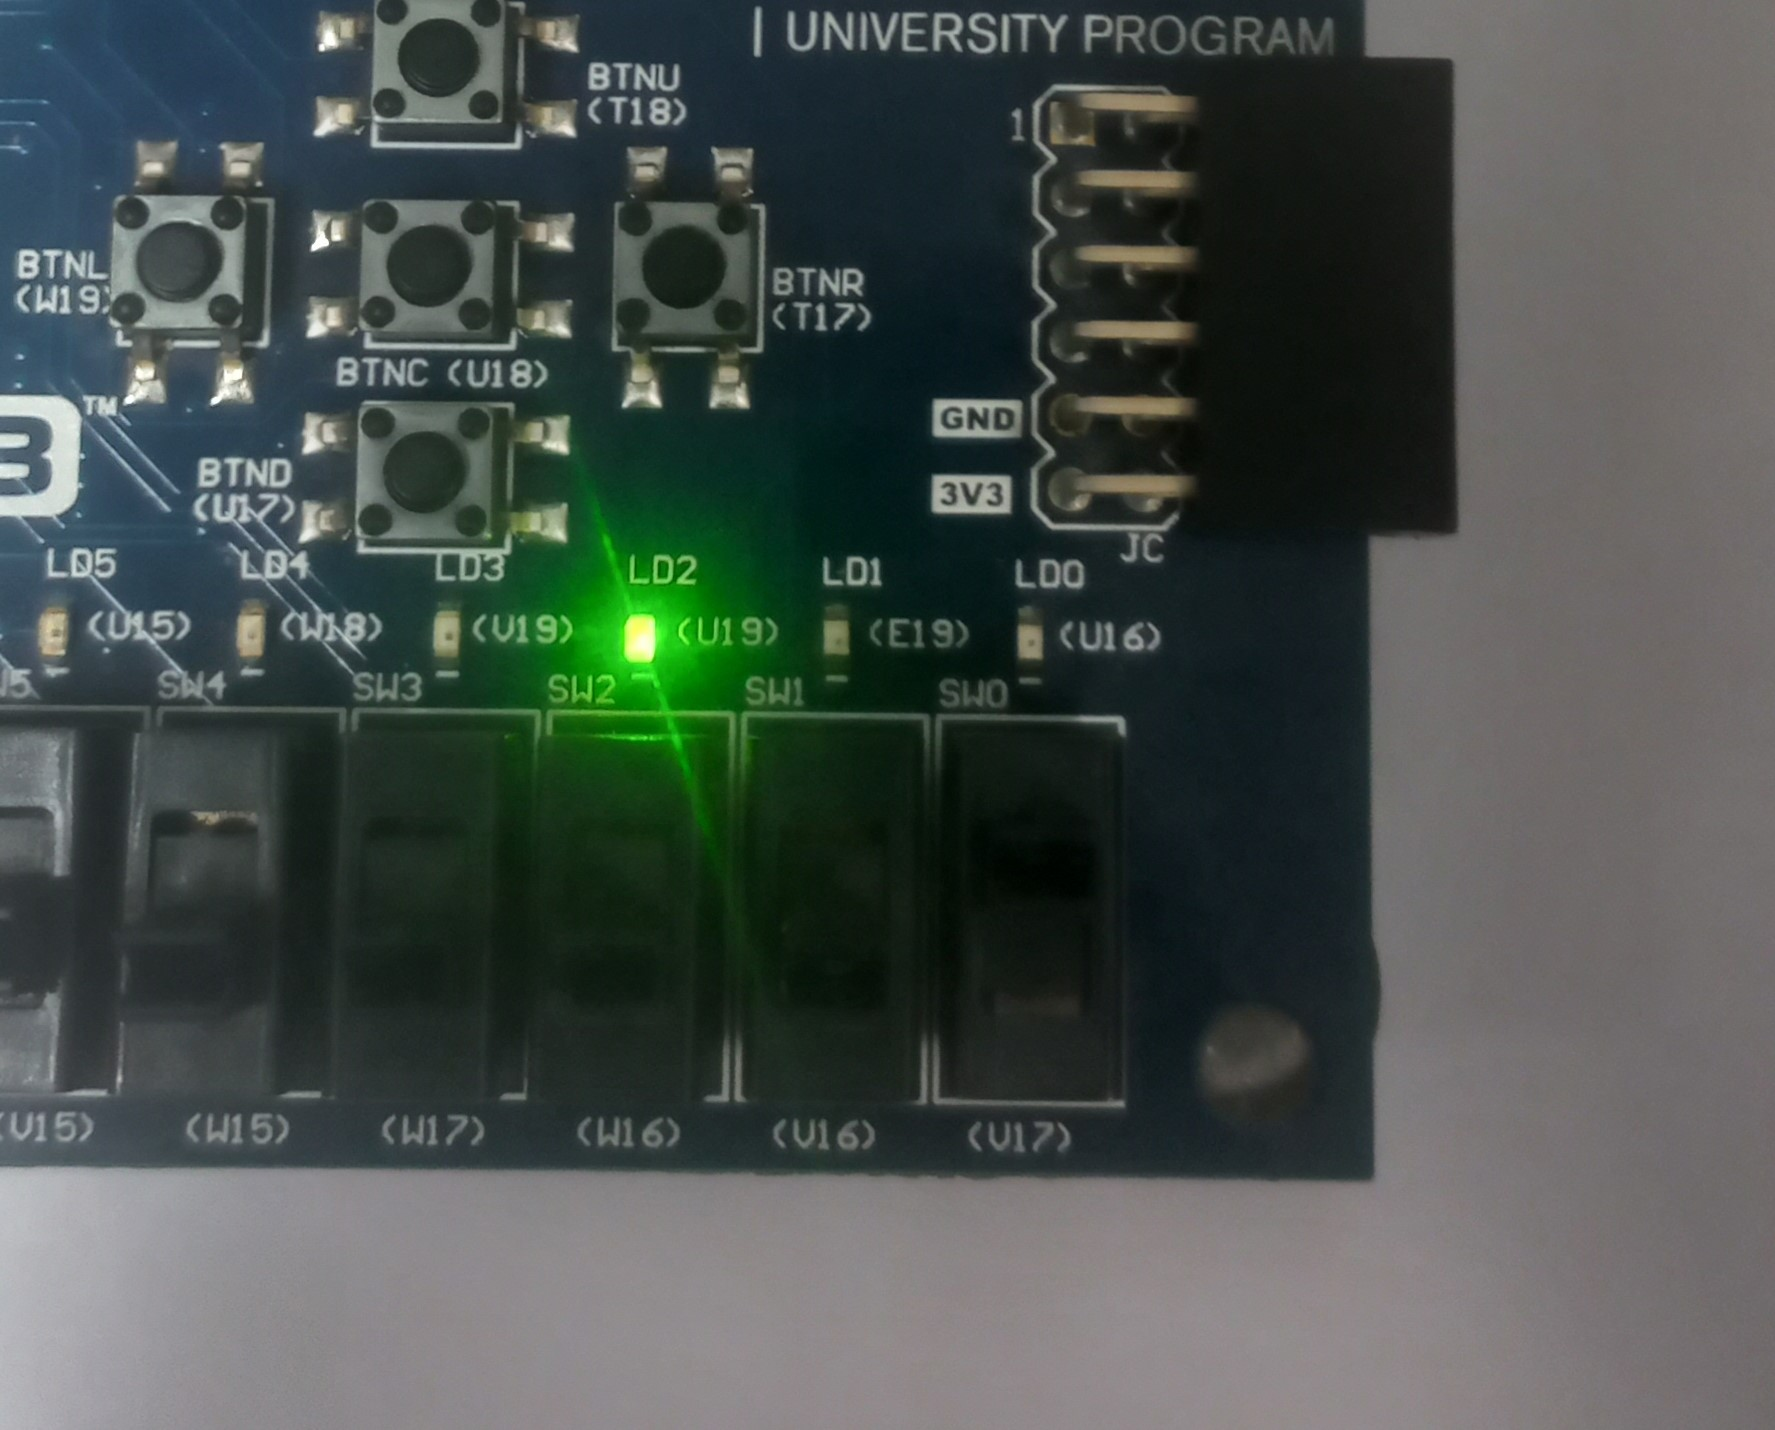
\includegraphics[width=0.4\linewidth]{simulations/magnitud-comp/comp-mag-10.jpg}
\end{figure}

Para la figura 8, se está cumpliendo la condición de AeqB es por eso que está prendido el led 0.
\begin{figure}[!ht]
    \centering
    \caption{A está en 1 y B está en 1}
    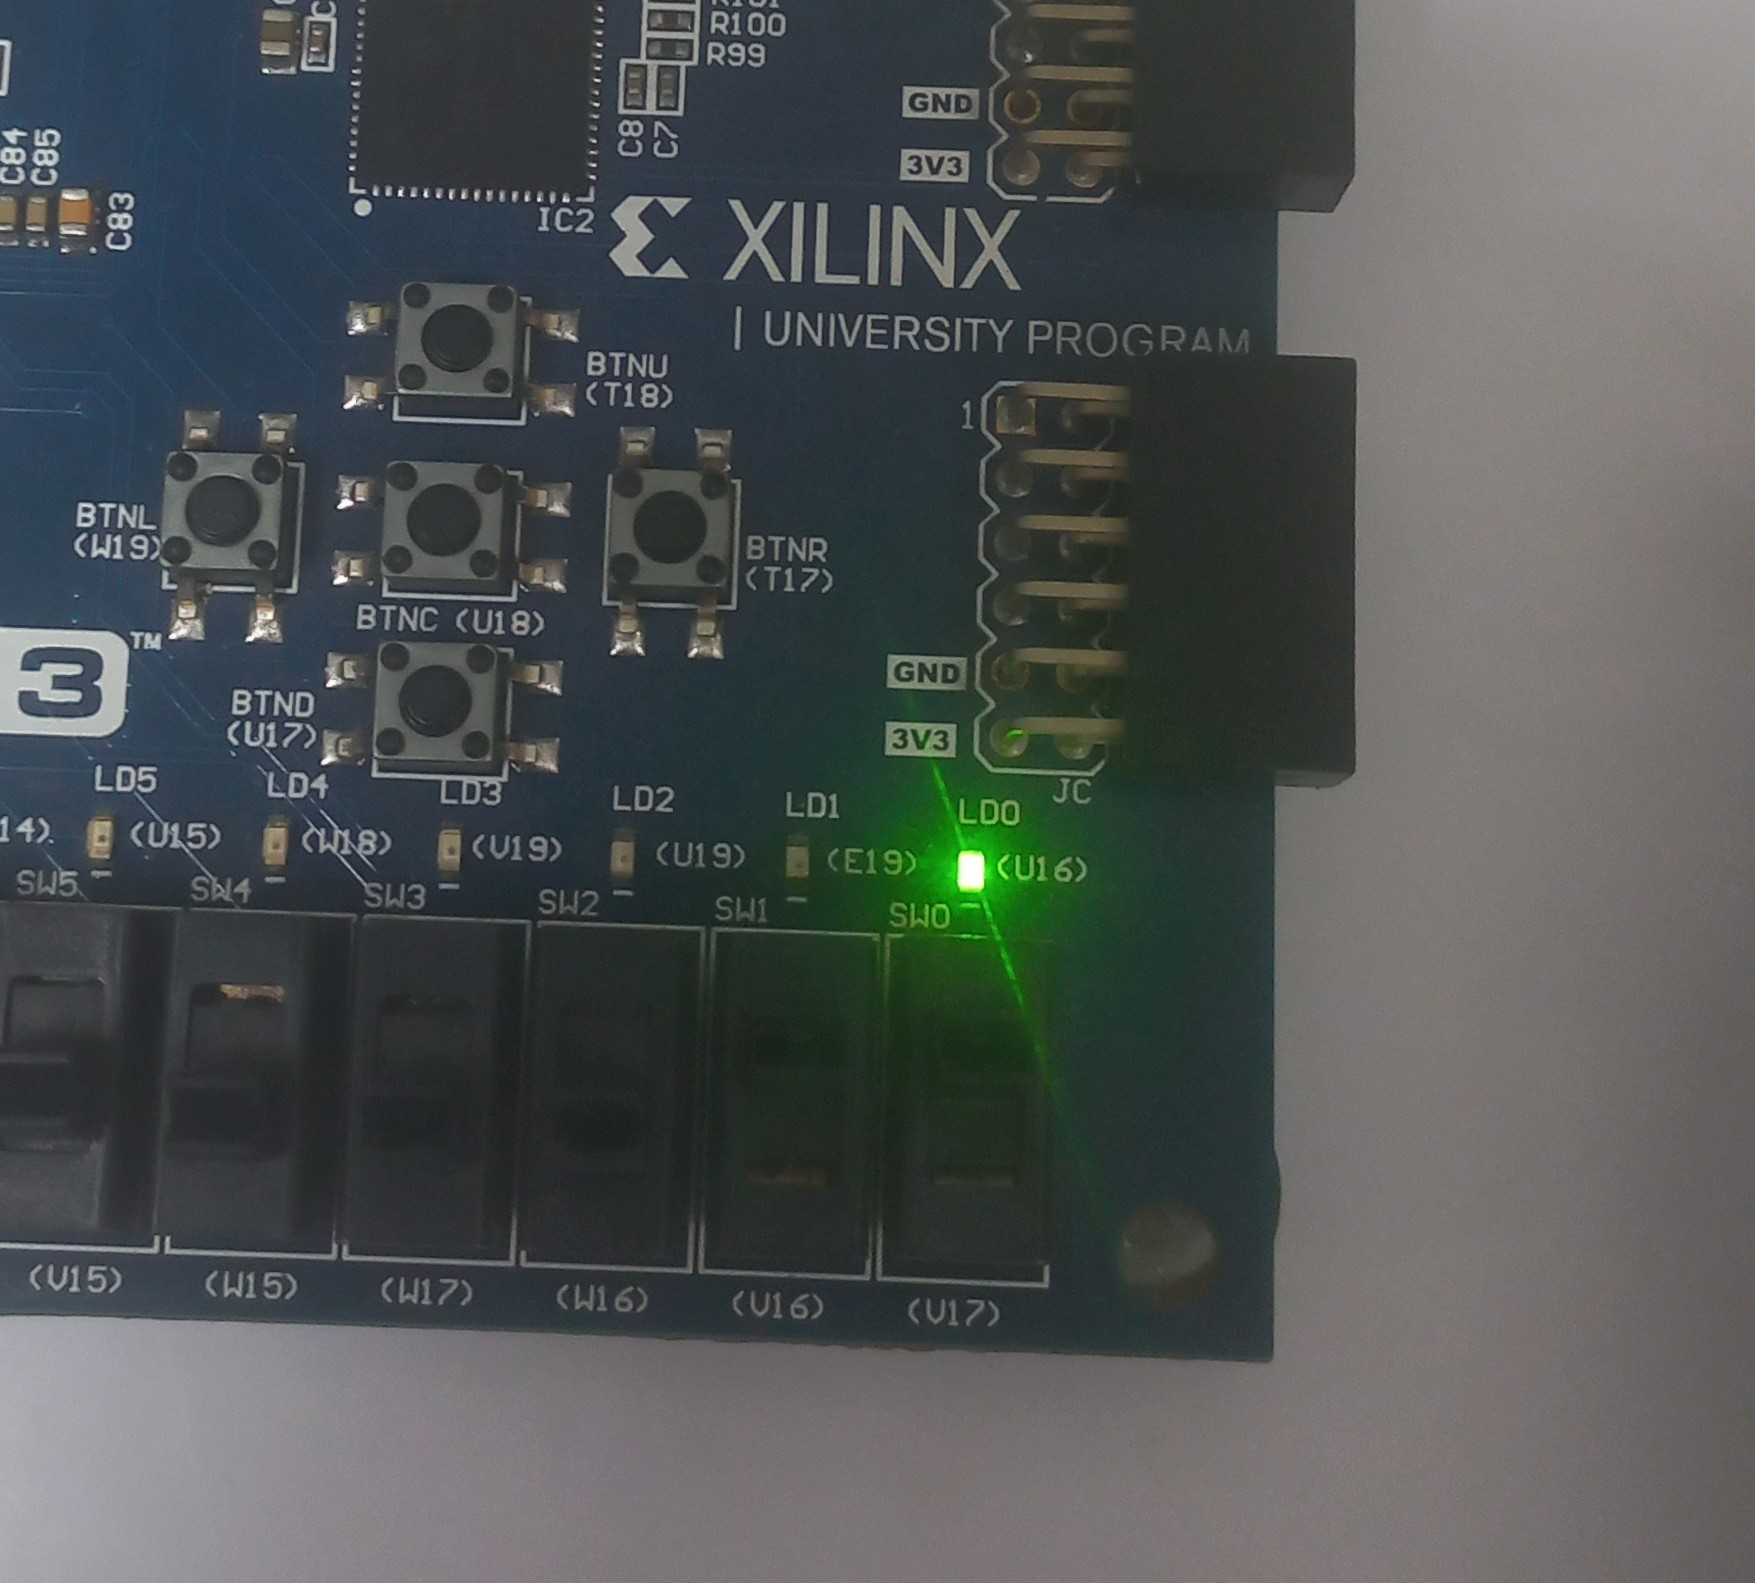
\includegraphics[width=0.4\linewidth]{simulations/magnitud-comp/comp.mag-11.jpg}
\end{figure}

Todas las fotos del circuito en el anexo.

\subsubsection*{Demultiplexor}
En el demultiplexor, para las dos entradas designamos que el switch 1 fuera A y el switch 0 fuera S. Para las salidas, Y0 sería el led 0 y para Y1 sería el led 1.

En la figura 9, como A está en cero aunque S esté en 1, ningún led va a prender.
\newpage
\begin{figure}[!ht]
    \centering
    \caption{Demultiplexor en A=0, S=1}
    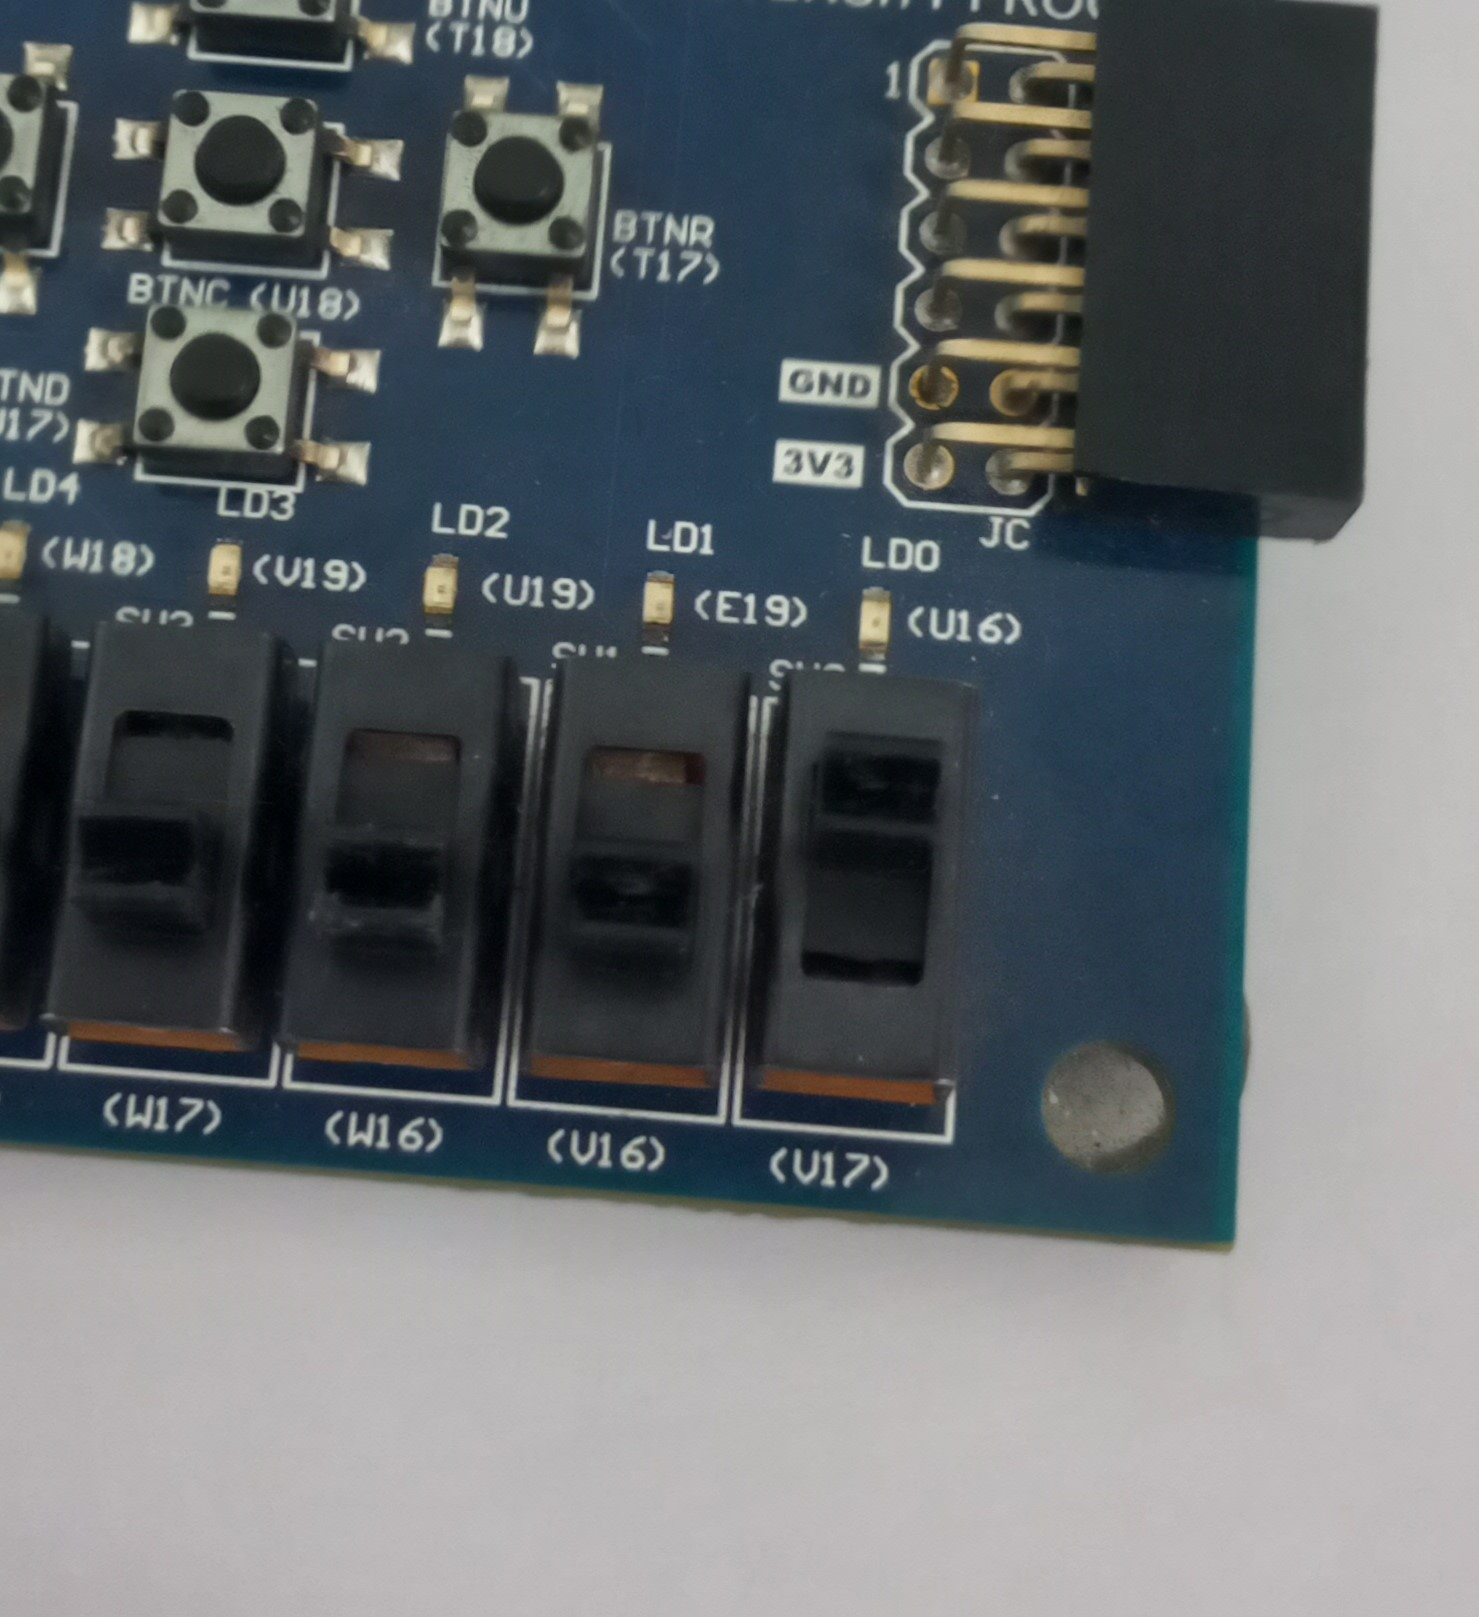
\includegraphics[width=0.4\linewidth]{simulations/demux/demux-01.jpg}
\end{figure}

Para la figura 10, el led 0 está prendido porque se está cumpliendo la condición de que A está en 1 y el canal de selección también está en 1.

\begin{figure}[!ht]
    \centering
    \caption{Demultiplexor en A=1, S=1}
    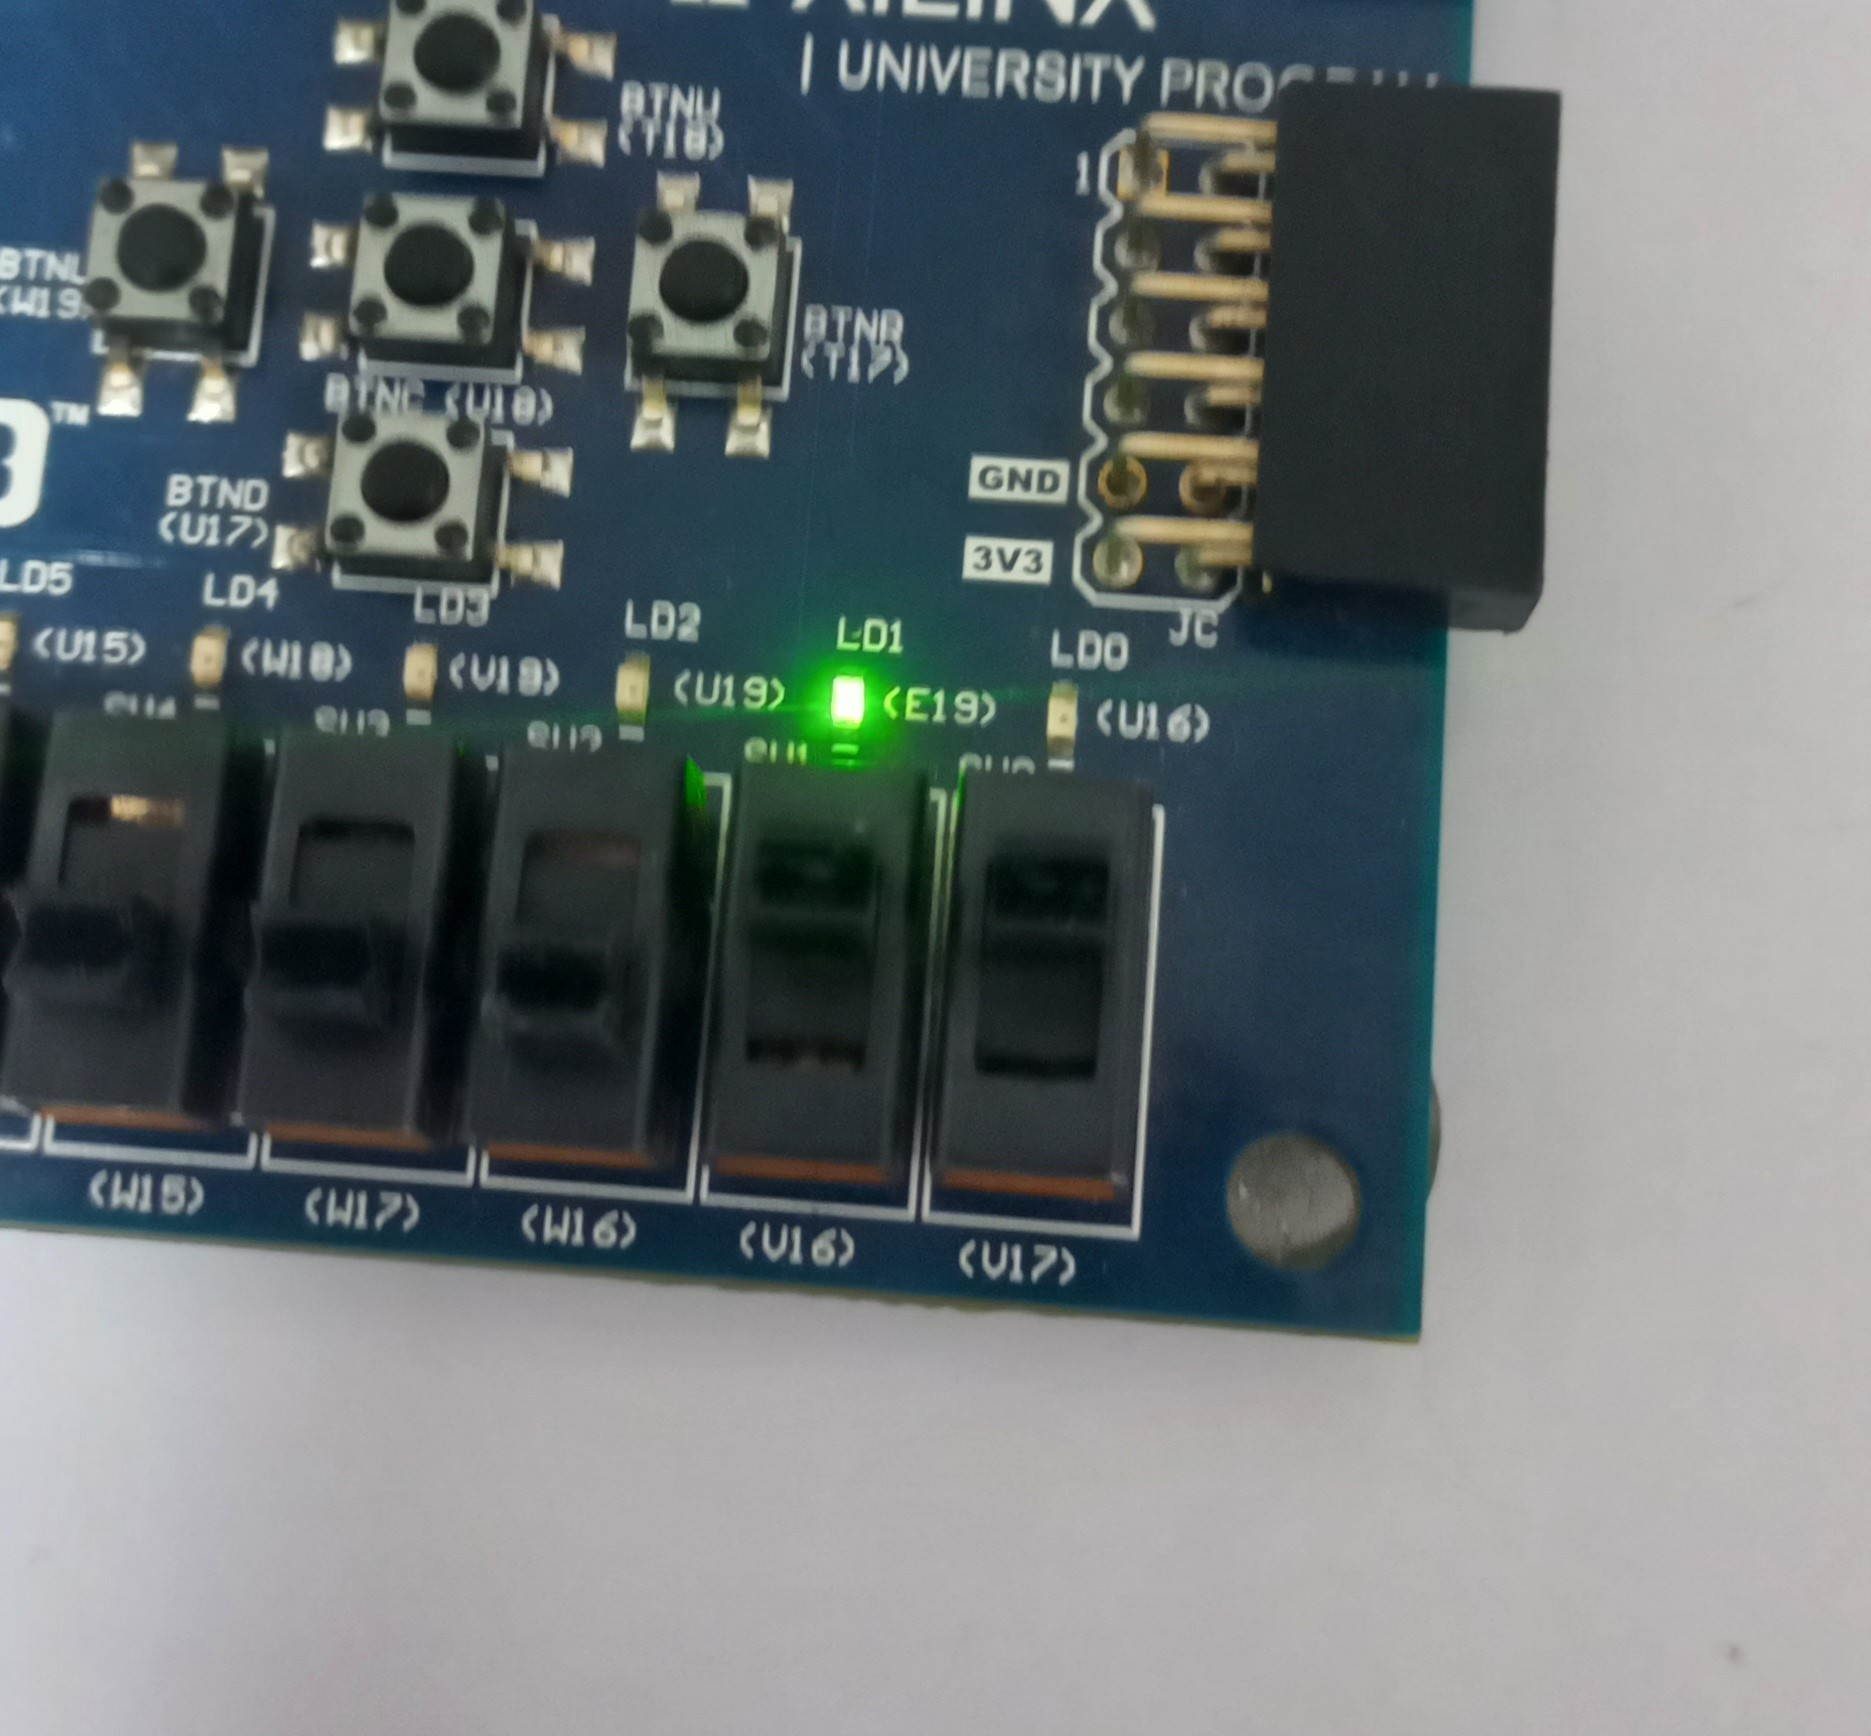
\includegraphics[width=0.5\linewidth]{simulations/demux/demux-11.jpg}
\end{figure}
Todas las fotos del circuito en el anexo.

\subsection{Conclusión}
En esta práctica logramos diseñar e implementar cuatro diferentes tipos de circuitos combinaciones, primero haciendo una lógica dependiendo de sus tablas de verdad, después de esto armando un código que nos permitiera ver su comportamiento en cada punto para después implementar este código en un circuito ya físico.

Los circuitos que nosotros diseñamos fueron un medio restador, un multiplexor, un comparador de magnitud y un demultiplexor. Como empezamos a construyendo la tabla de verdad de cada circuito, a partir de esto fuimos armando sus códigos ya que dependiendo de los casos para algunos era mejor desarrollar sus códigos a partir de su comportamiento o de condicionales. Ya una vez armado el código pudimos ver a partir de su testbench su comportamiento y ver si coincidía con la tabla de verdad, una vez que coincidían ambas podíamos pasar todo esto a un circuito físico, en este caso usamos un Basys 3, en este logramos comprobar que efectivamente todo funcionaba correctamente. 

Igual vimos que es más complicado ubicar un error en una Basys 3 y corregirlo que en un protoboard ya que en un protoboard puedes cambiar de nodo pero en una Basys 3 necesitas cambiar de placa. Igualmente uno debe seleccionar correctamente todos los pasos de programación. Aun así, es más rápido ejecutar las pruebas físicas y eso lo convierte en una gran ventaja a la hora de hacer malos cálculos y corregirlos. 

\newpage %Termina la pagina y empieza una nueva
\appendix % A partir de este comando, todas las secciones por venir serán parte del apéndice

\subsection*{Imágenes completas}

\subsubsection*{Medio Restador}
\begin{figure}[!ht]
    \centering
    \caption{Medio restador en A=0, B=0}
    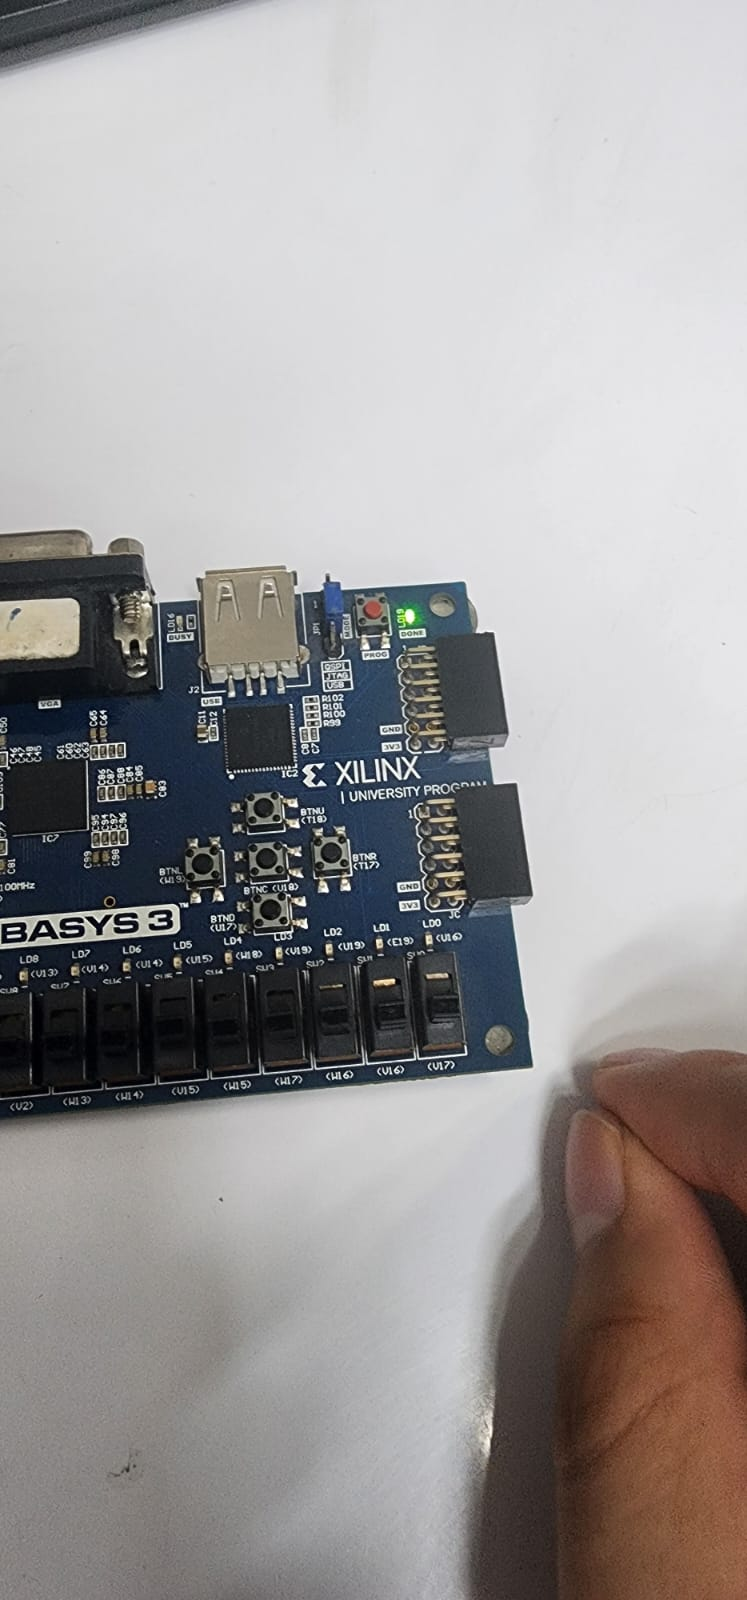
\includegraphics[width=0.4\linewidth]{simulations/half/half0.jpg}
\end{figure}
\newpage
\begin{figure}[!ht]
    \centering
    \caption{Medio restador en A=1, B=0}
    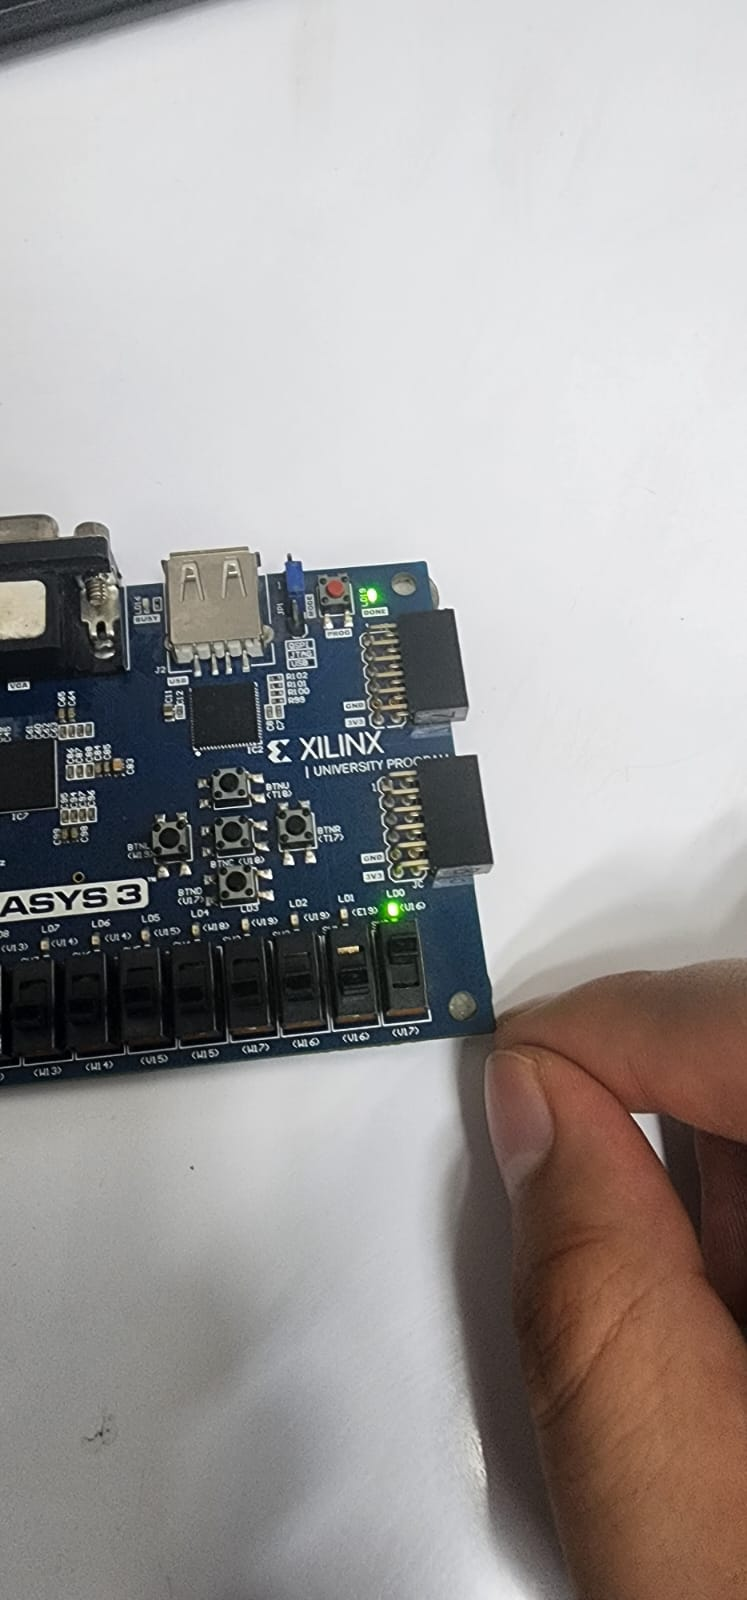
\includegraphics[width=0.4\linewidth]{simulations/half/half1.jpg}
\end{figure}
\newpage
\begin{figure}[!ht]
    \centering
    \caption{Medio restador en A=0, B=1}
    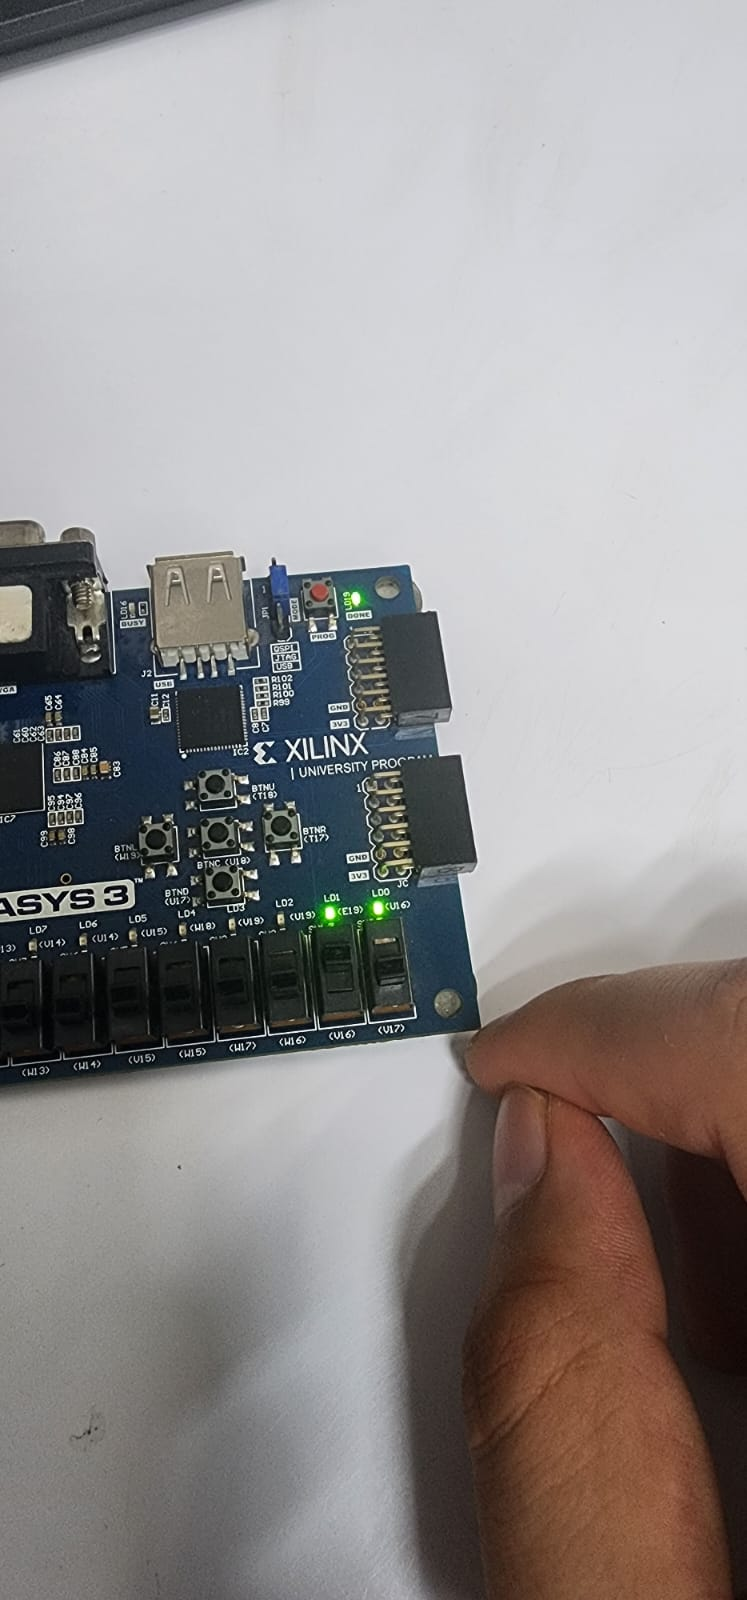
\includegraphics[width=0.4\linewidth]{simulations/half/half2.jpg}
\end{figure}
\newpage
\begin{figure}[!ht]
    \centering
    \caption{Medio restador en A=1, B=1}
    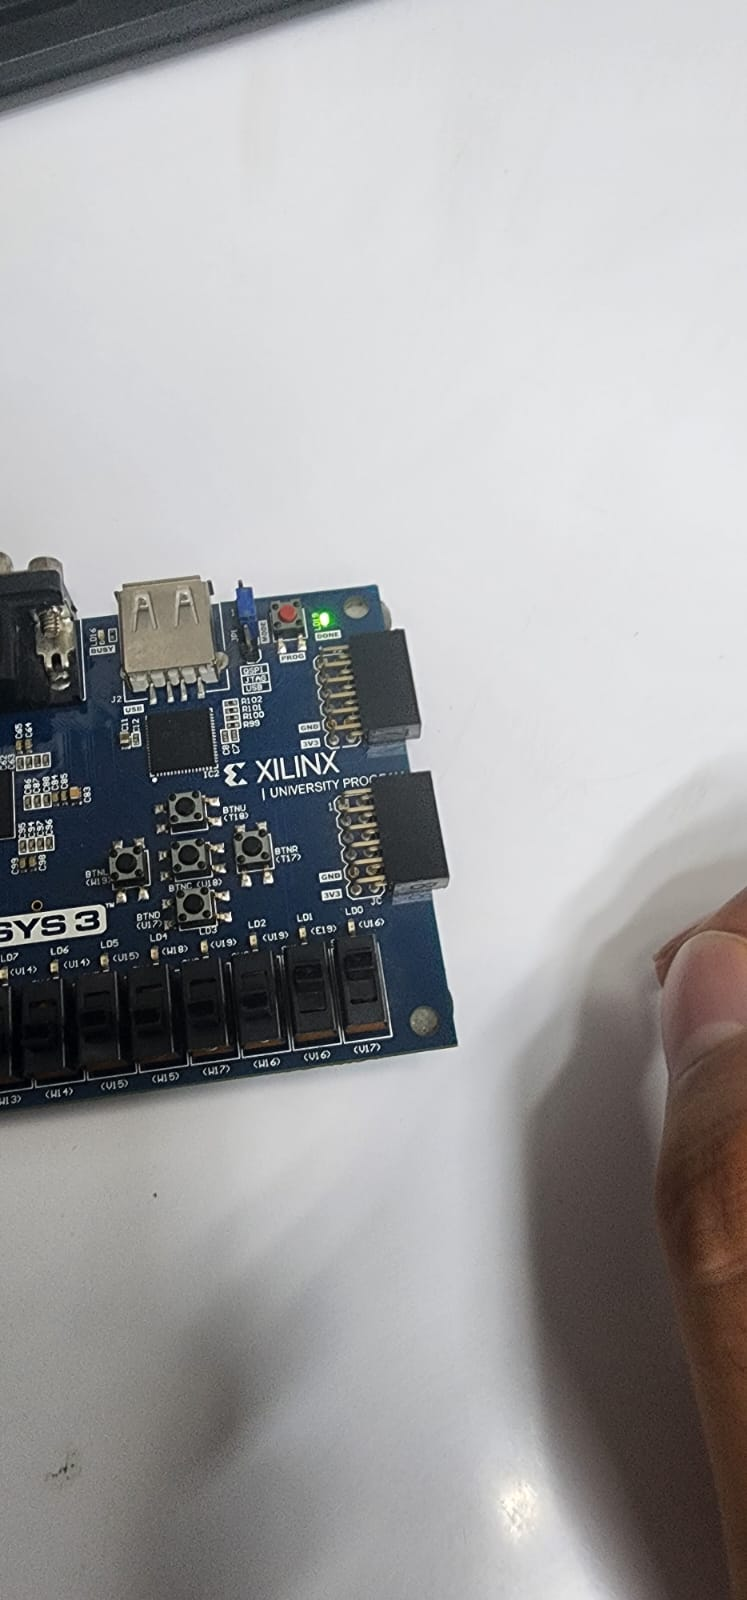
\includegraphics[width=0.4\linewidth]{simulations/half/half3.jpg}
\end{figure}
\newpage

\subsubsection*{Multiplexor}

\begin{figure}[!ht]
    \centering
    \caption{Multiplexor en A=0, B=0, S=0}
    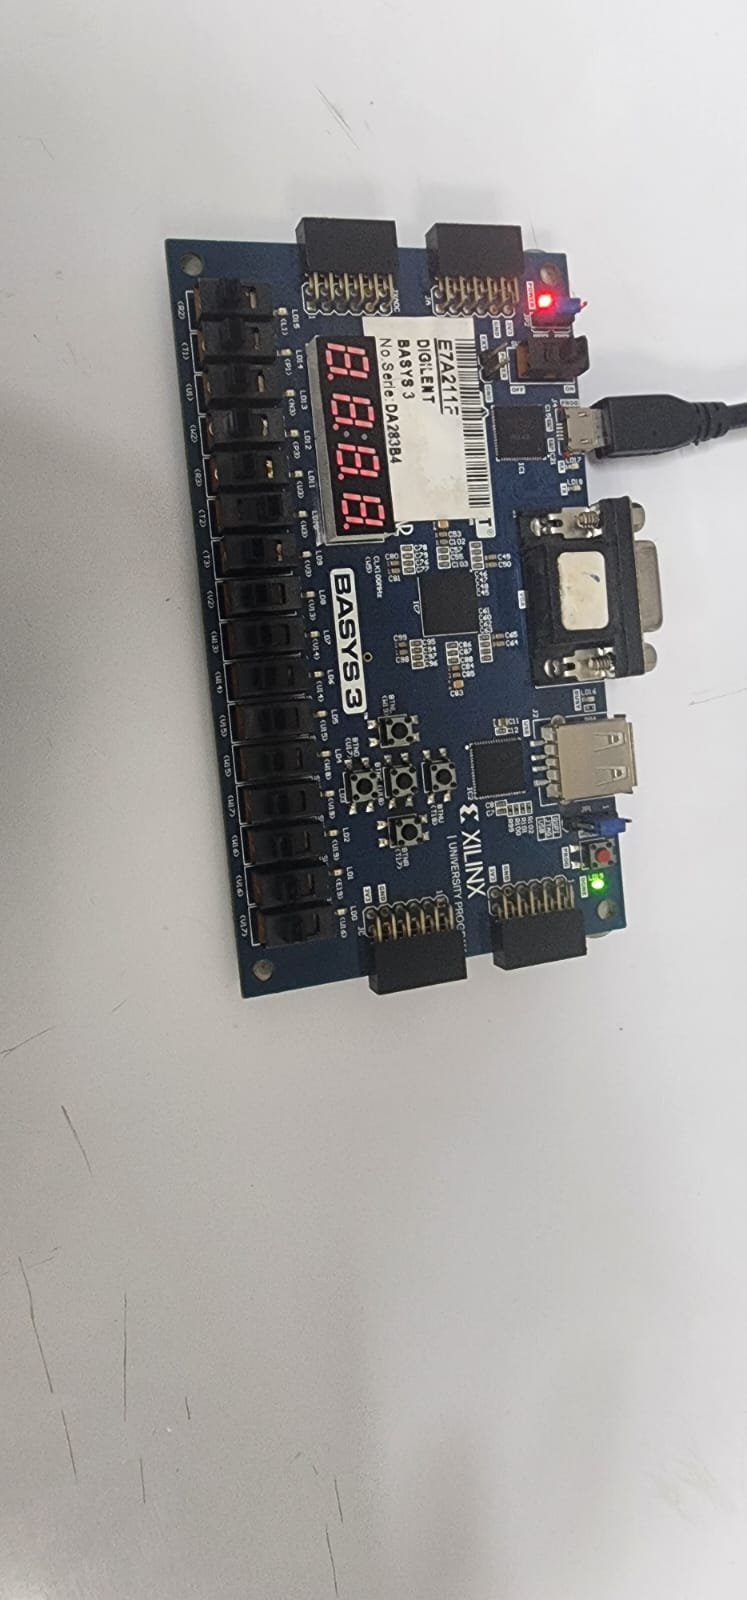
\includegraphics[width=0.5\linewidth]{simulations/multiplex/multiplex0.jpg}
\end{figure}
\newpage
\begin{figure}[!ht]
    \centering
    \caption{Multiplexor en A=0, B=1, S=0}
    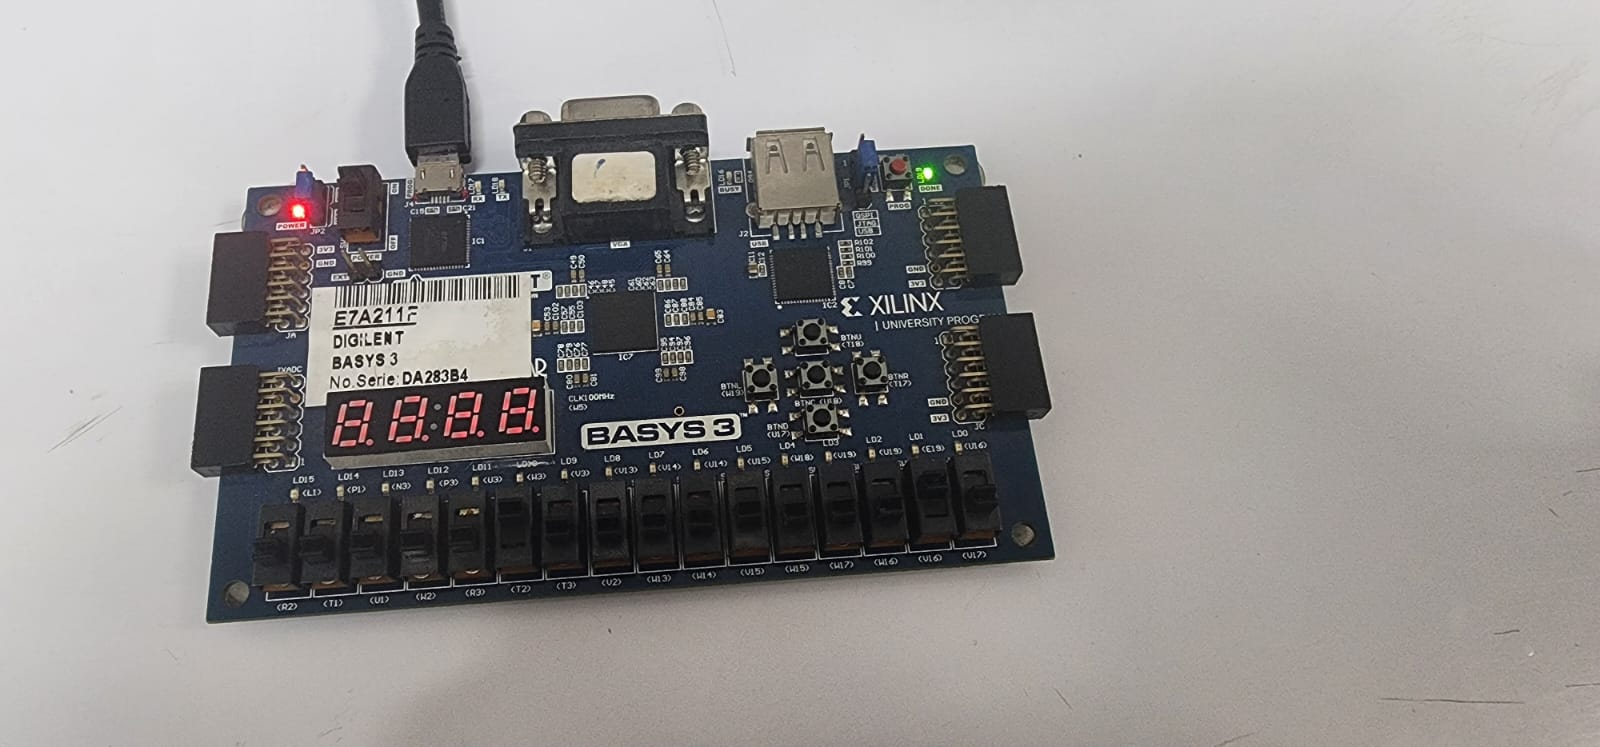
\includegraphics[width=1\linewidth]{simulations/multiplex/multiplex1.jpg}
\end{figure}
\begin{figure}[!ht]
    \centering
    \caption{Multiplexor en A=1, B=0, S=0}
    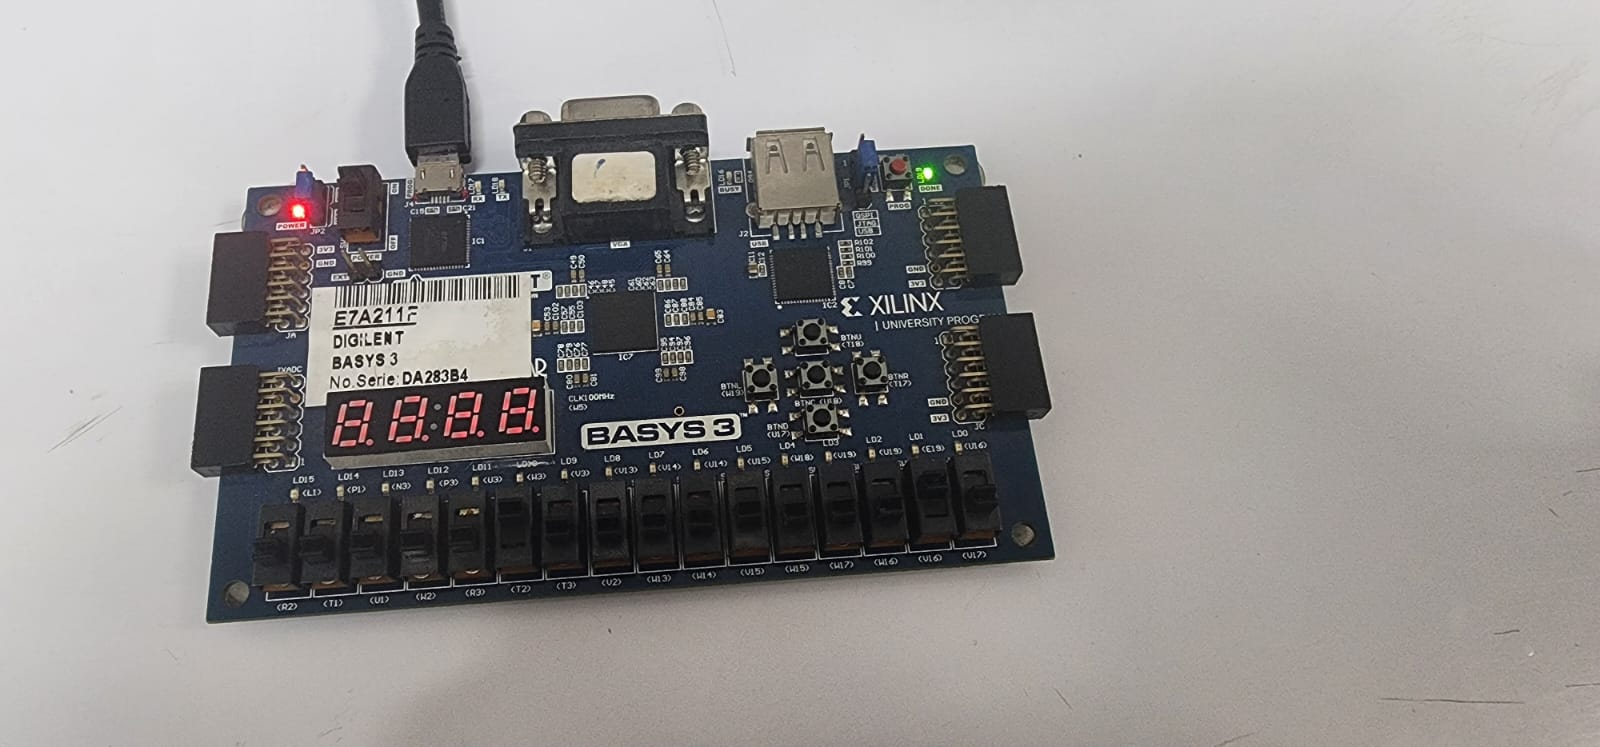
\includegraphics[width=1\linewidth]{simulations/multiplex/multiplex1.jpg}
\end{figure}
\newpage

\begin{figure}[!ht]
    \centering
    \caption{Multiplexor en A=1, B=1, S=0}
    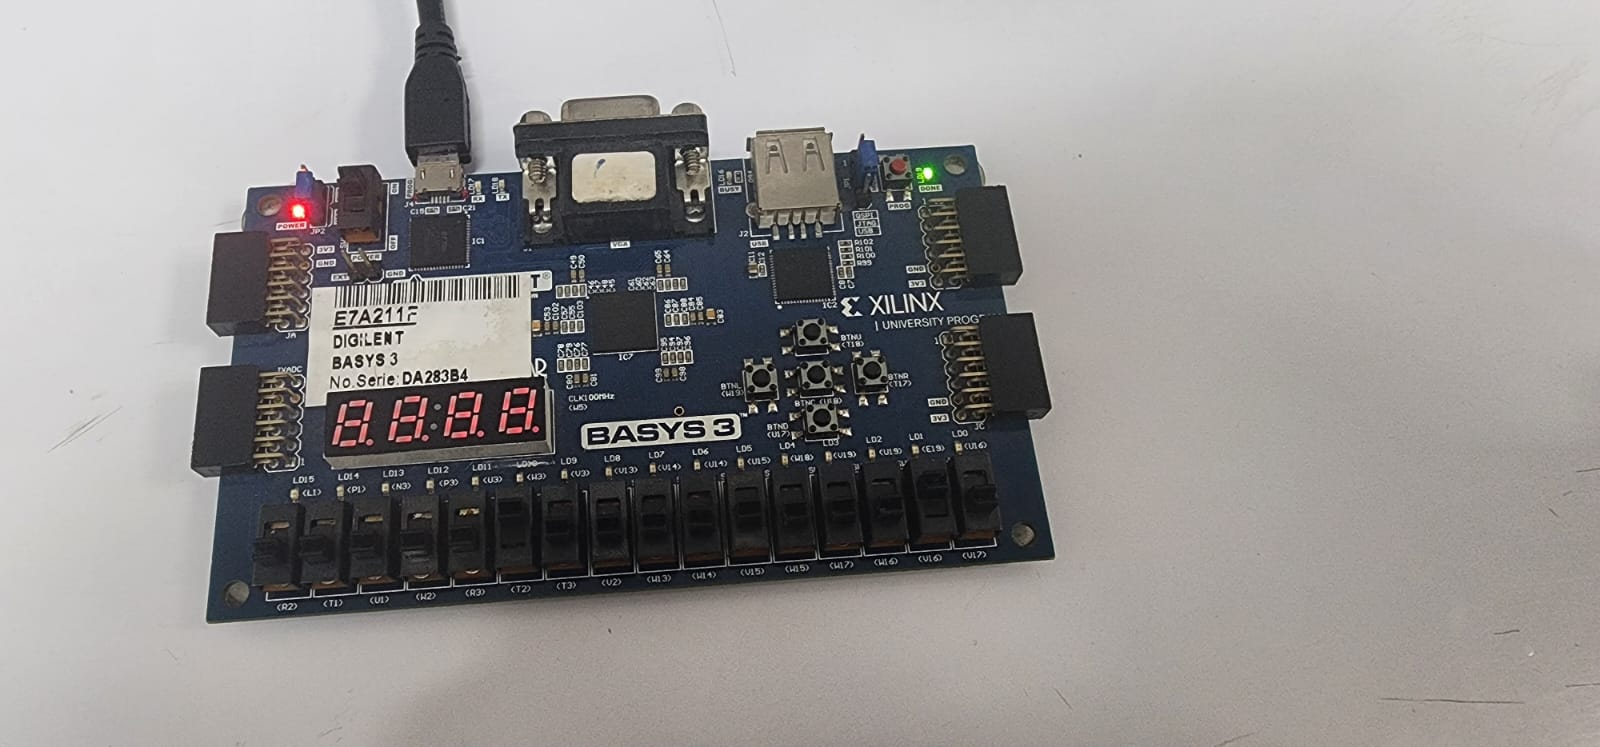
\includegraphics[width=1\linewidth]{simulations/multiplex/multiplex1.jpg}
\end{figure}
\begin{figure}[!ht]
    \centering
    \caption{Multiplexor en A=0, B=0, S=1}
    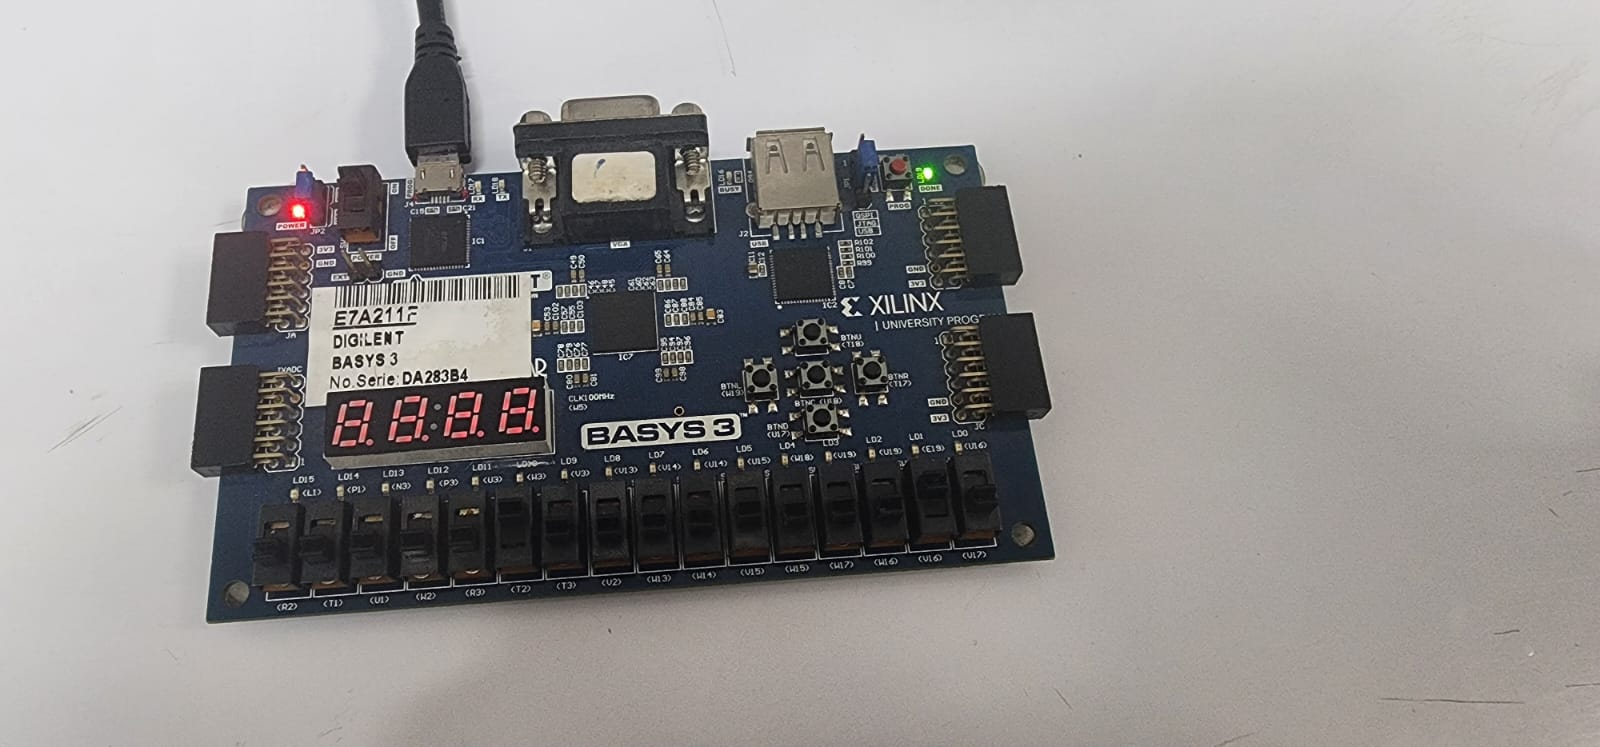
\includegraphics[width=1\linewidth]{simulations/multiplex/multiplex1.jpg}
\end{figure}
\newpage

\begin{figure}[!ht]
    \centering
    \caption{Multiplexor en A=0, B=1, S=1}
    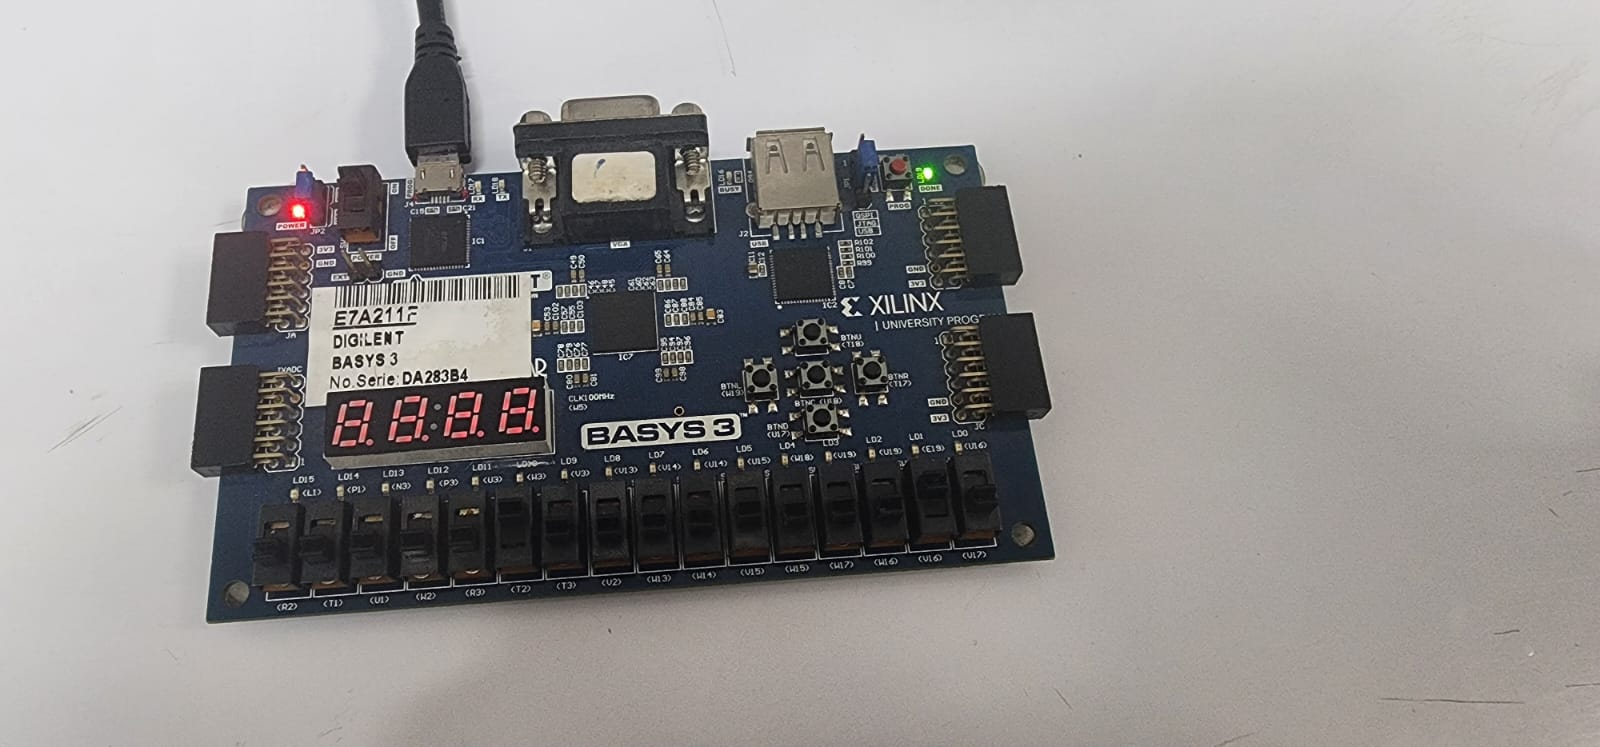
\includegraphics[width=1\linewidth]{simulations/multiplex/multiplex1.jpg}
\end{figure}
\begin{figure}[!ht]
    \centering
    \caption{Multiplexor en A=1, B=0, S=1}
    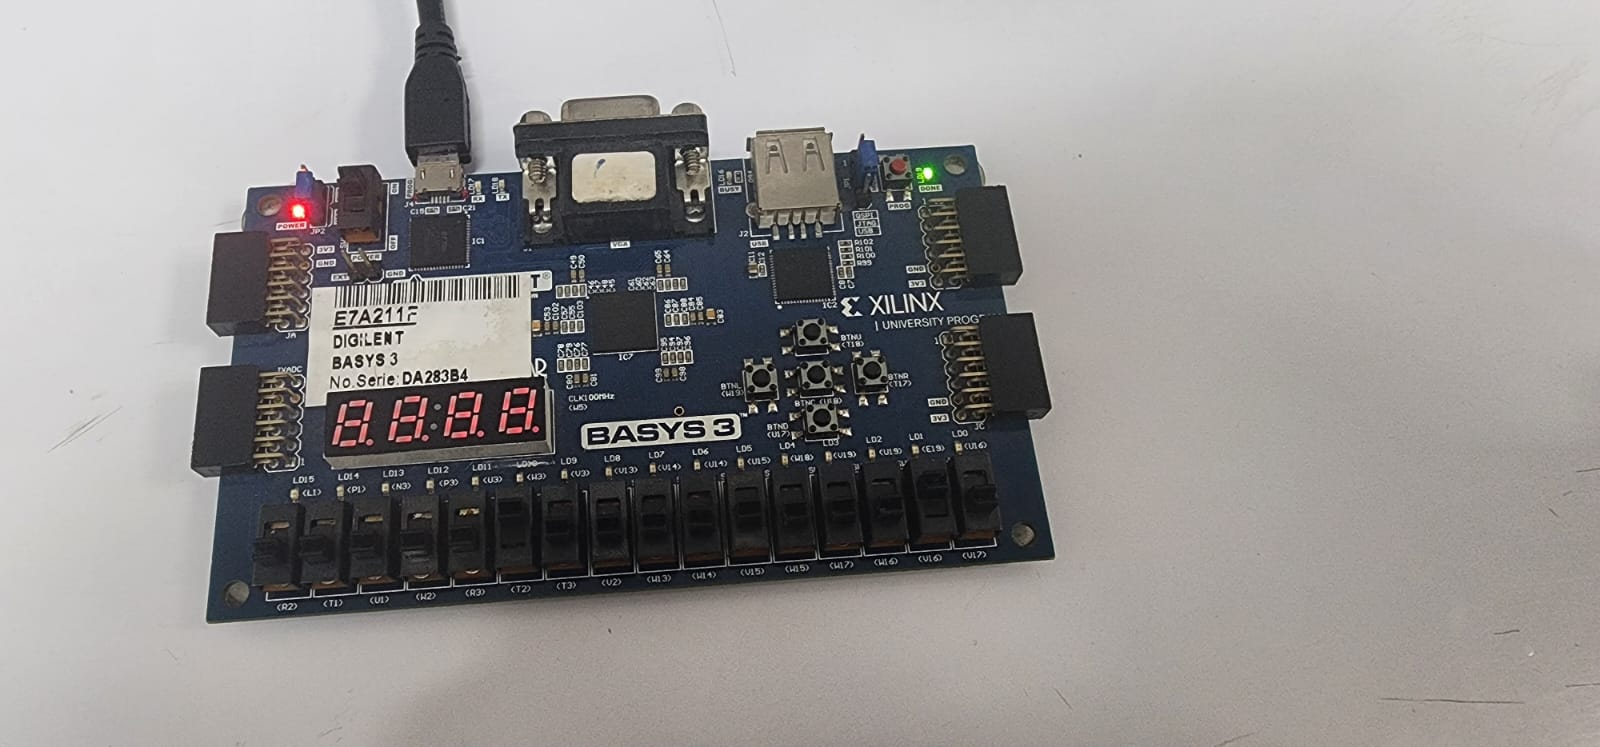
\includegraphics[width=1\linewidth]{simulations/multiplex/multiplex1.jpg}
\end{figure}
\newpage

\begin{figure}[!ht]
    \centering
    \caption{Multiplexor en A=1, B=1, S=1}
    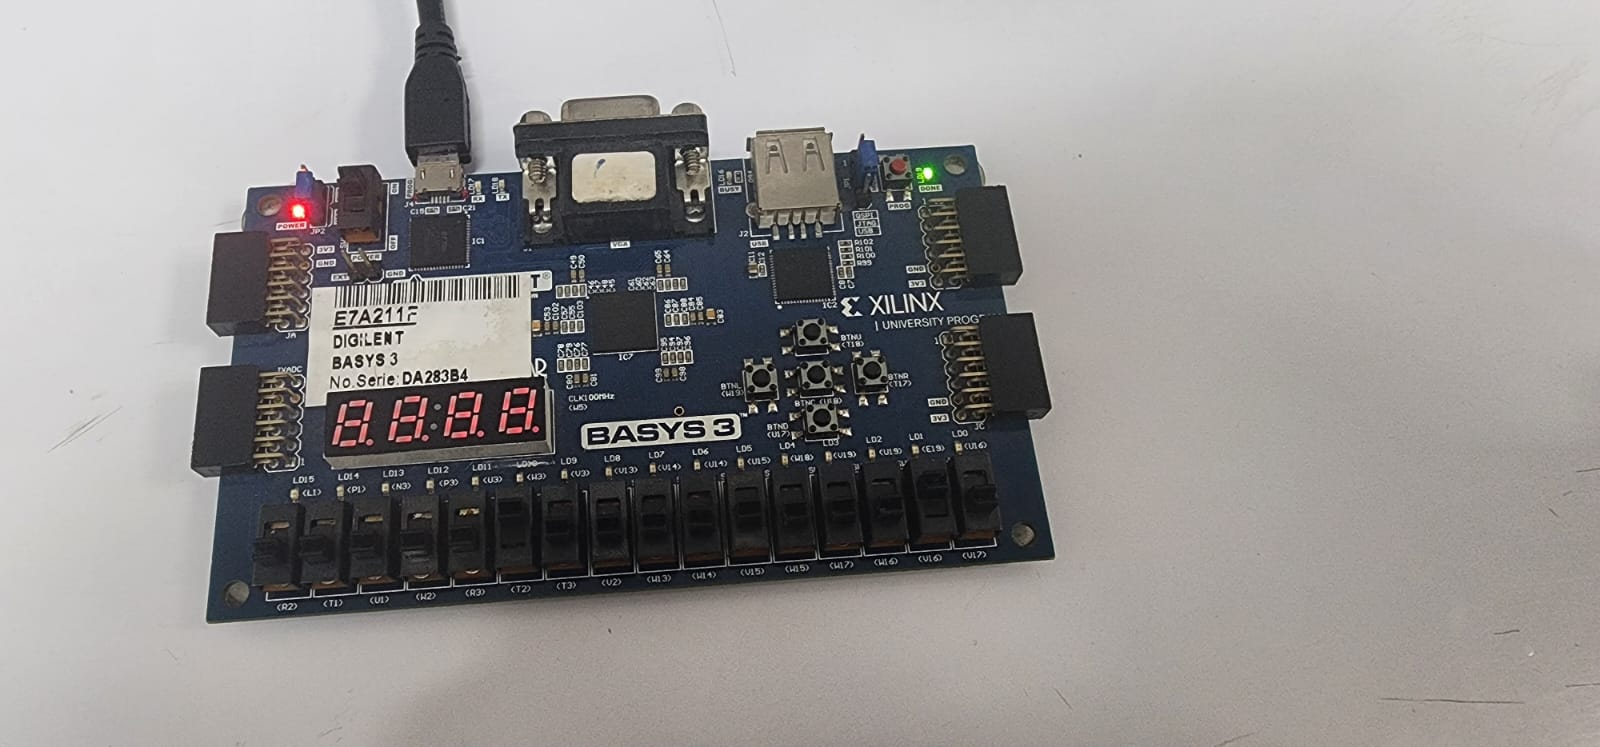
\includegraphics[width=1\linewidth]{simulations/multiplex/multiplex1.jpg}
\end{figure}
\newpage

\subsubsection*{Comparador de Magnitud}

\begin{figure}[!ht]
    \centering
    \caption{Comparador de magnitud en A=0, B=0}
    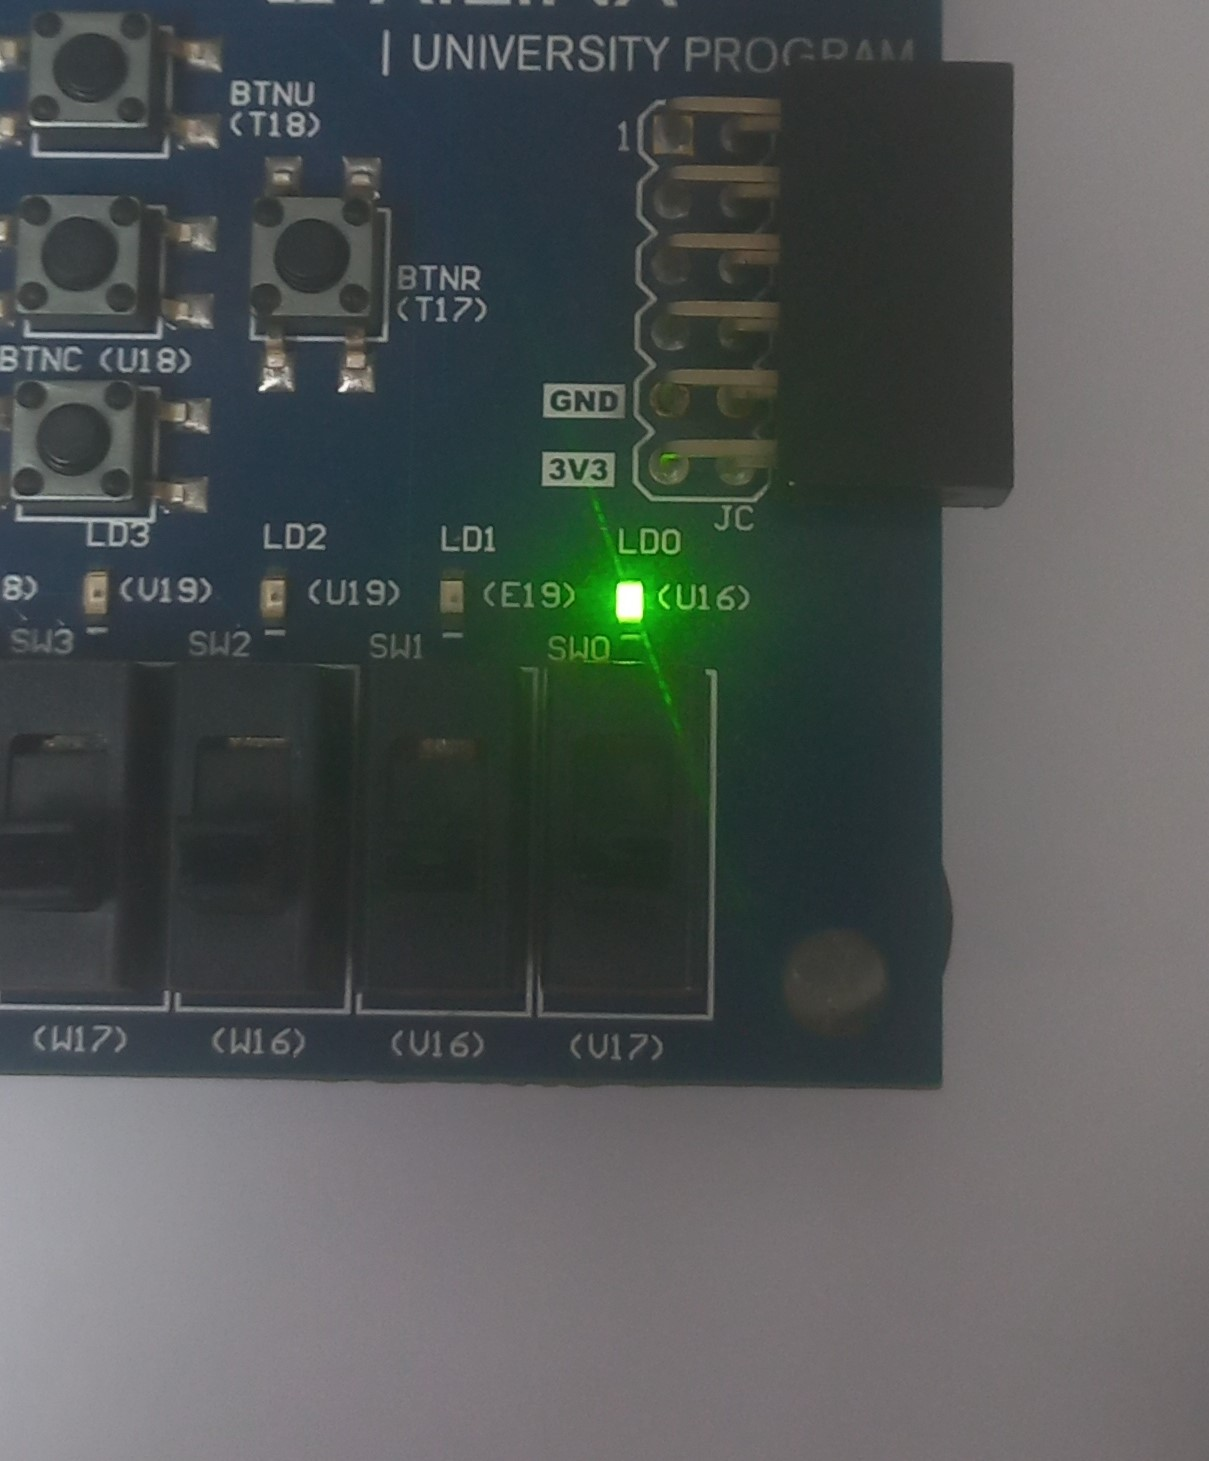
\includegraphics[width=0.4\linewidth]{simulations/magnitud-comp/comp-mag-00.jpg}
\end{figure}
\begin{figure}[!ht]
    \centering
    \caption{Comparador de magnitud en A=0, B=1}
    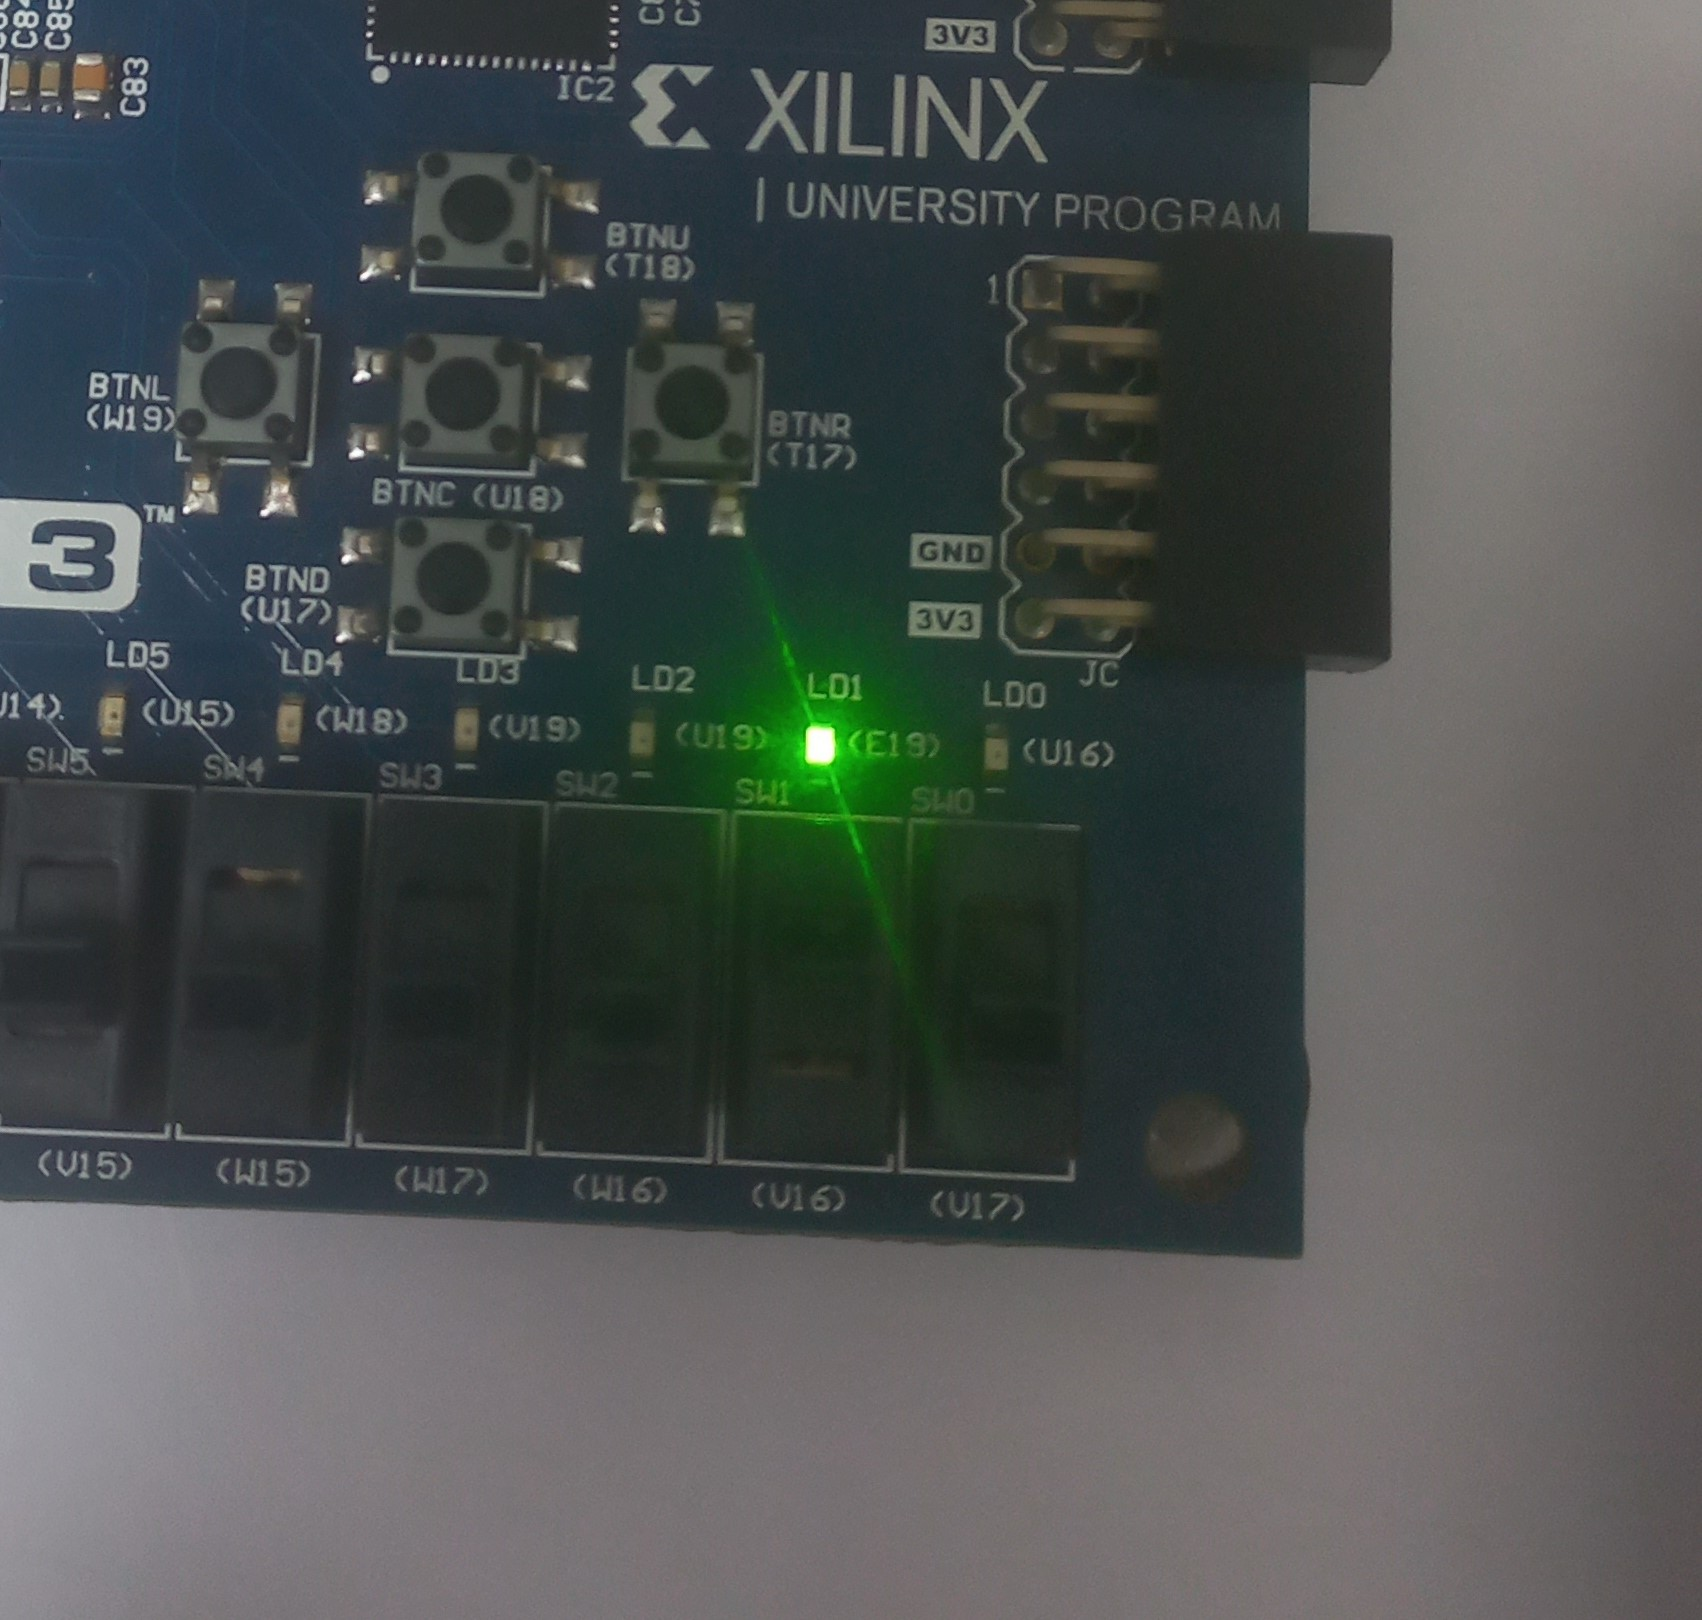
\includegraphics[width=0.5\linewidth]{simulations/magnitud-comp/comp-mag-01.jpg}
\end{figure}
\newpage

\begin{figure}[!ht]
    \centering
    \caption{Comparador de magnitud en A=1, B=0}
    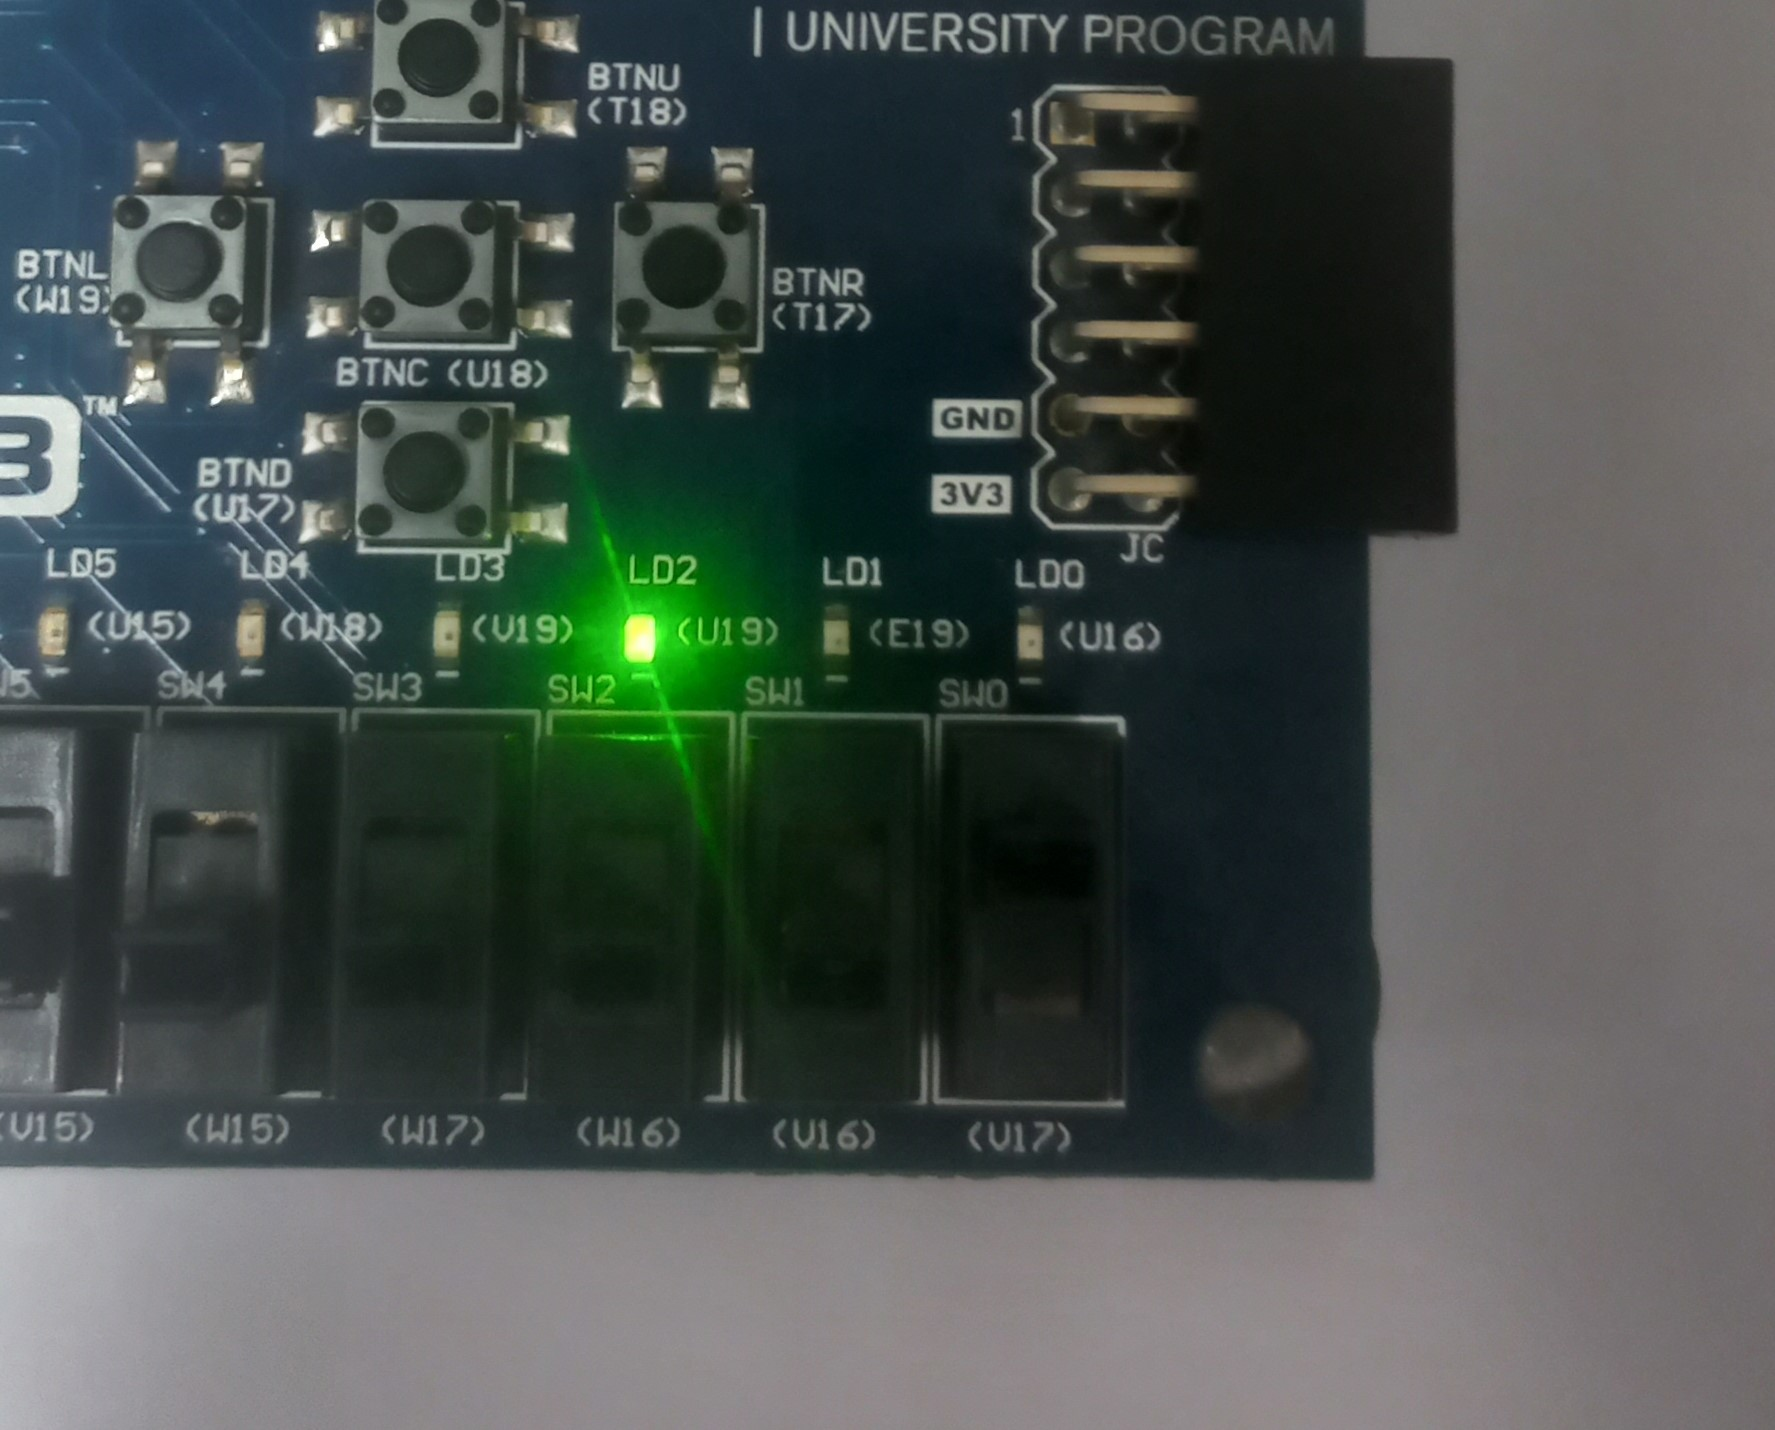
\includegraphics[width=0.5\linewidth]{simulations/magnitud-comp/comp-mag-10.jpg}
\end{figure}
\begin{figure}[!ht]
    \centering
    \caption{Comparador de magnitud en A=1, B=1}
    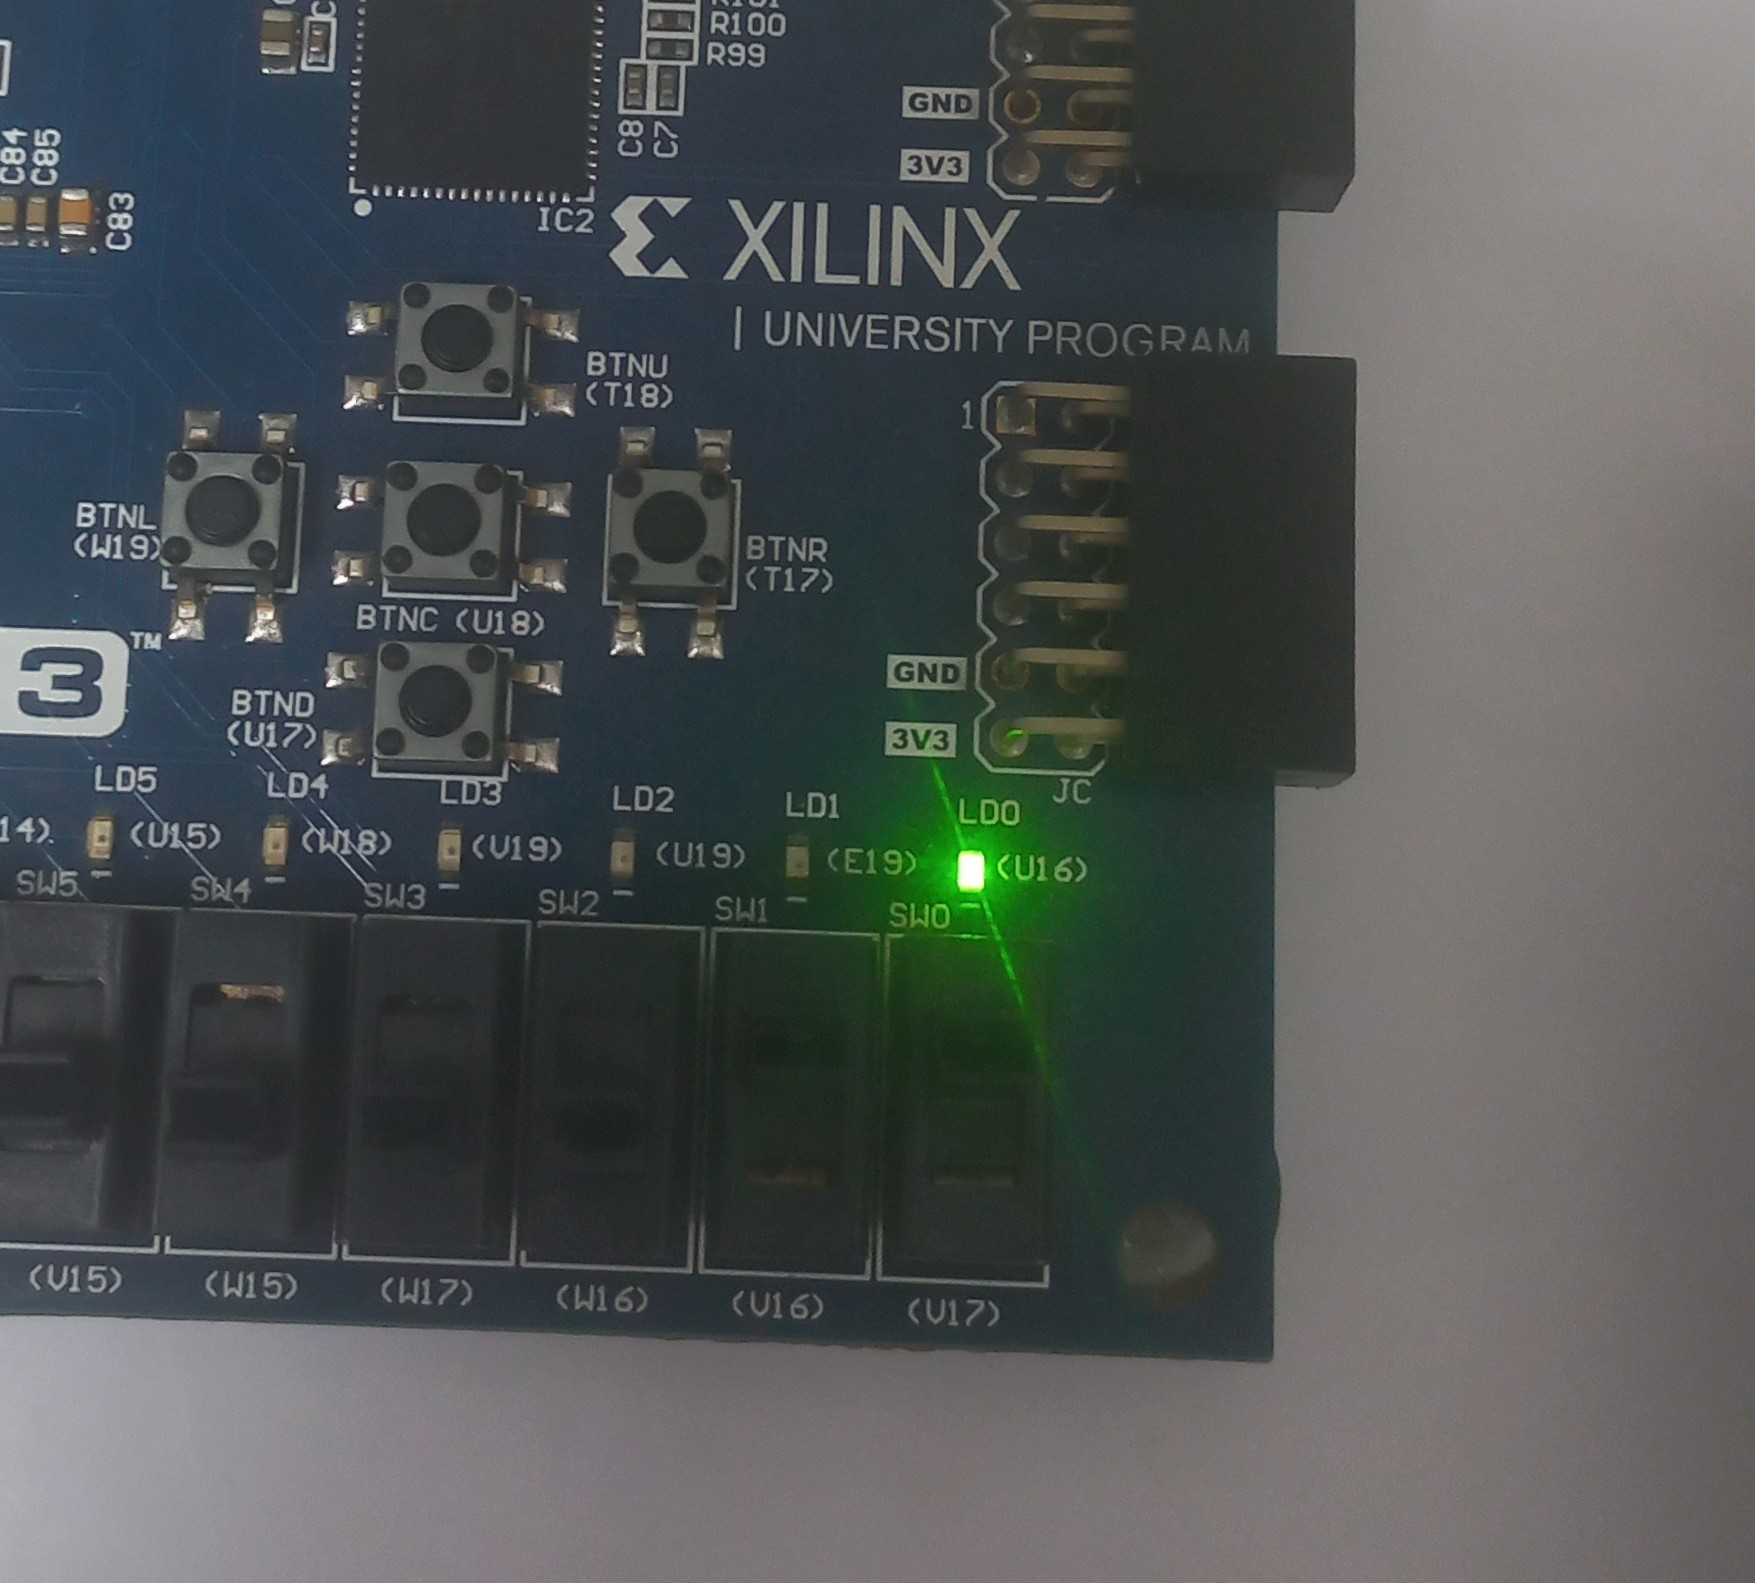
\includegraphics[width=0.5\linewidth]{simulations/magnitud-comp/comp.mag-11.jpg}
\end{figure}
\newpage

\subsubsection*{Demultiplexor}
\begin{figure}[!ht]
    \centering
    \caption{Demultiplexor en A=0, S=0}
    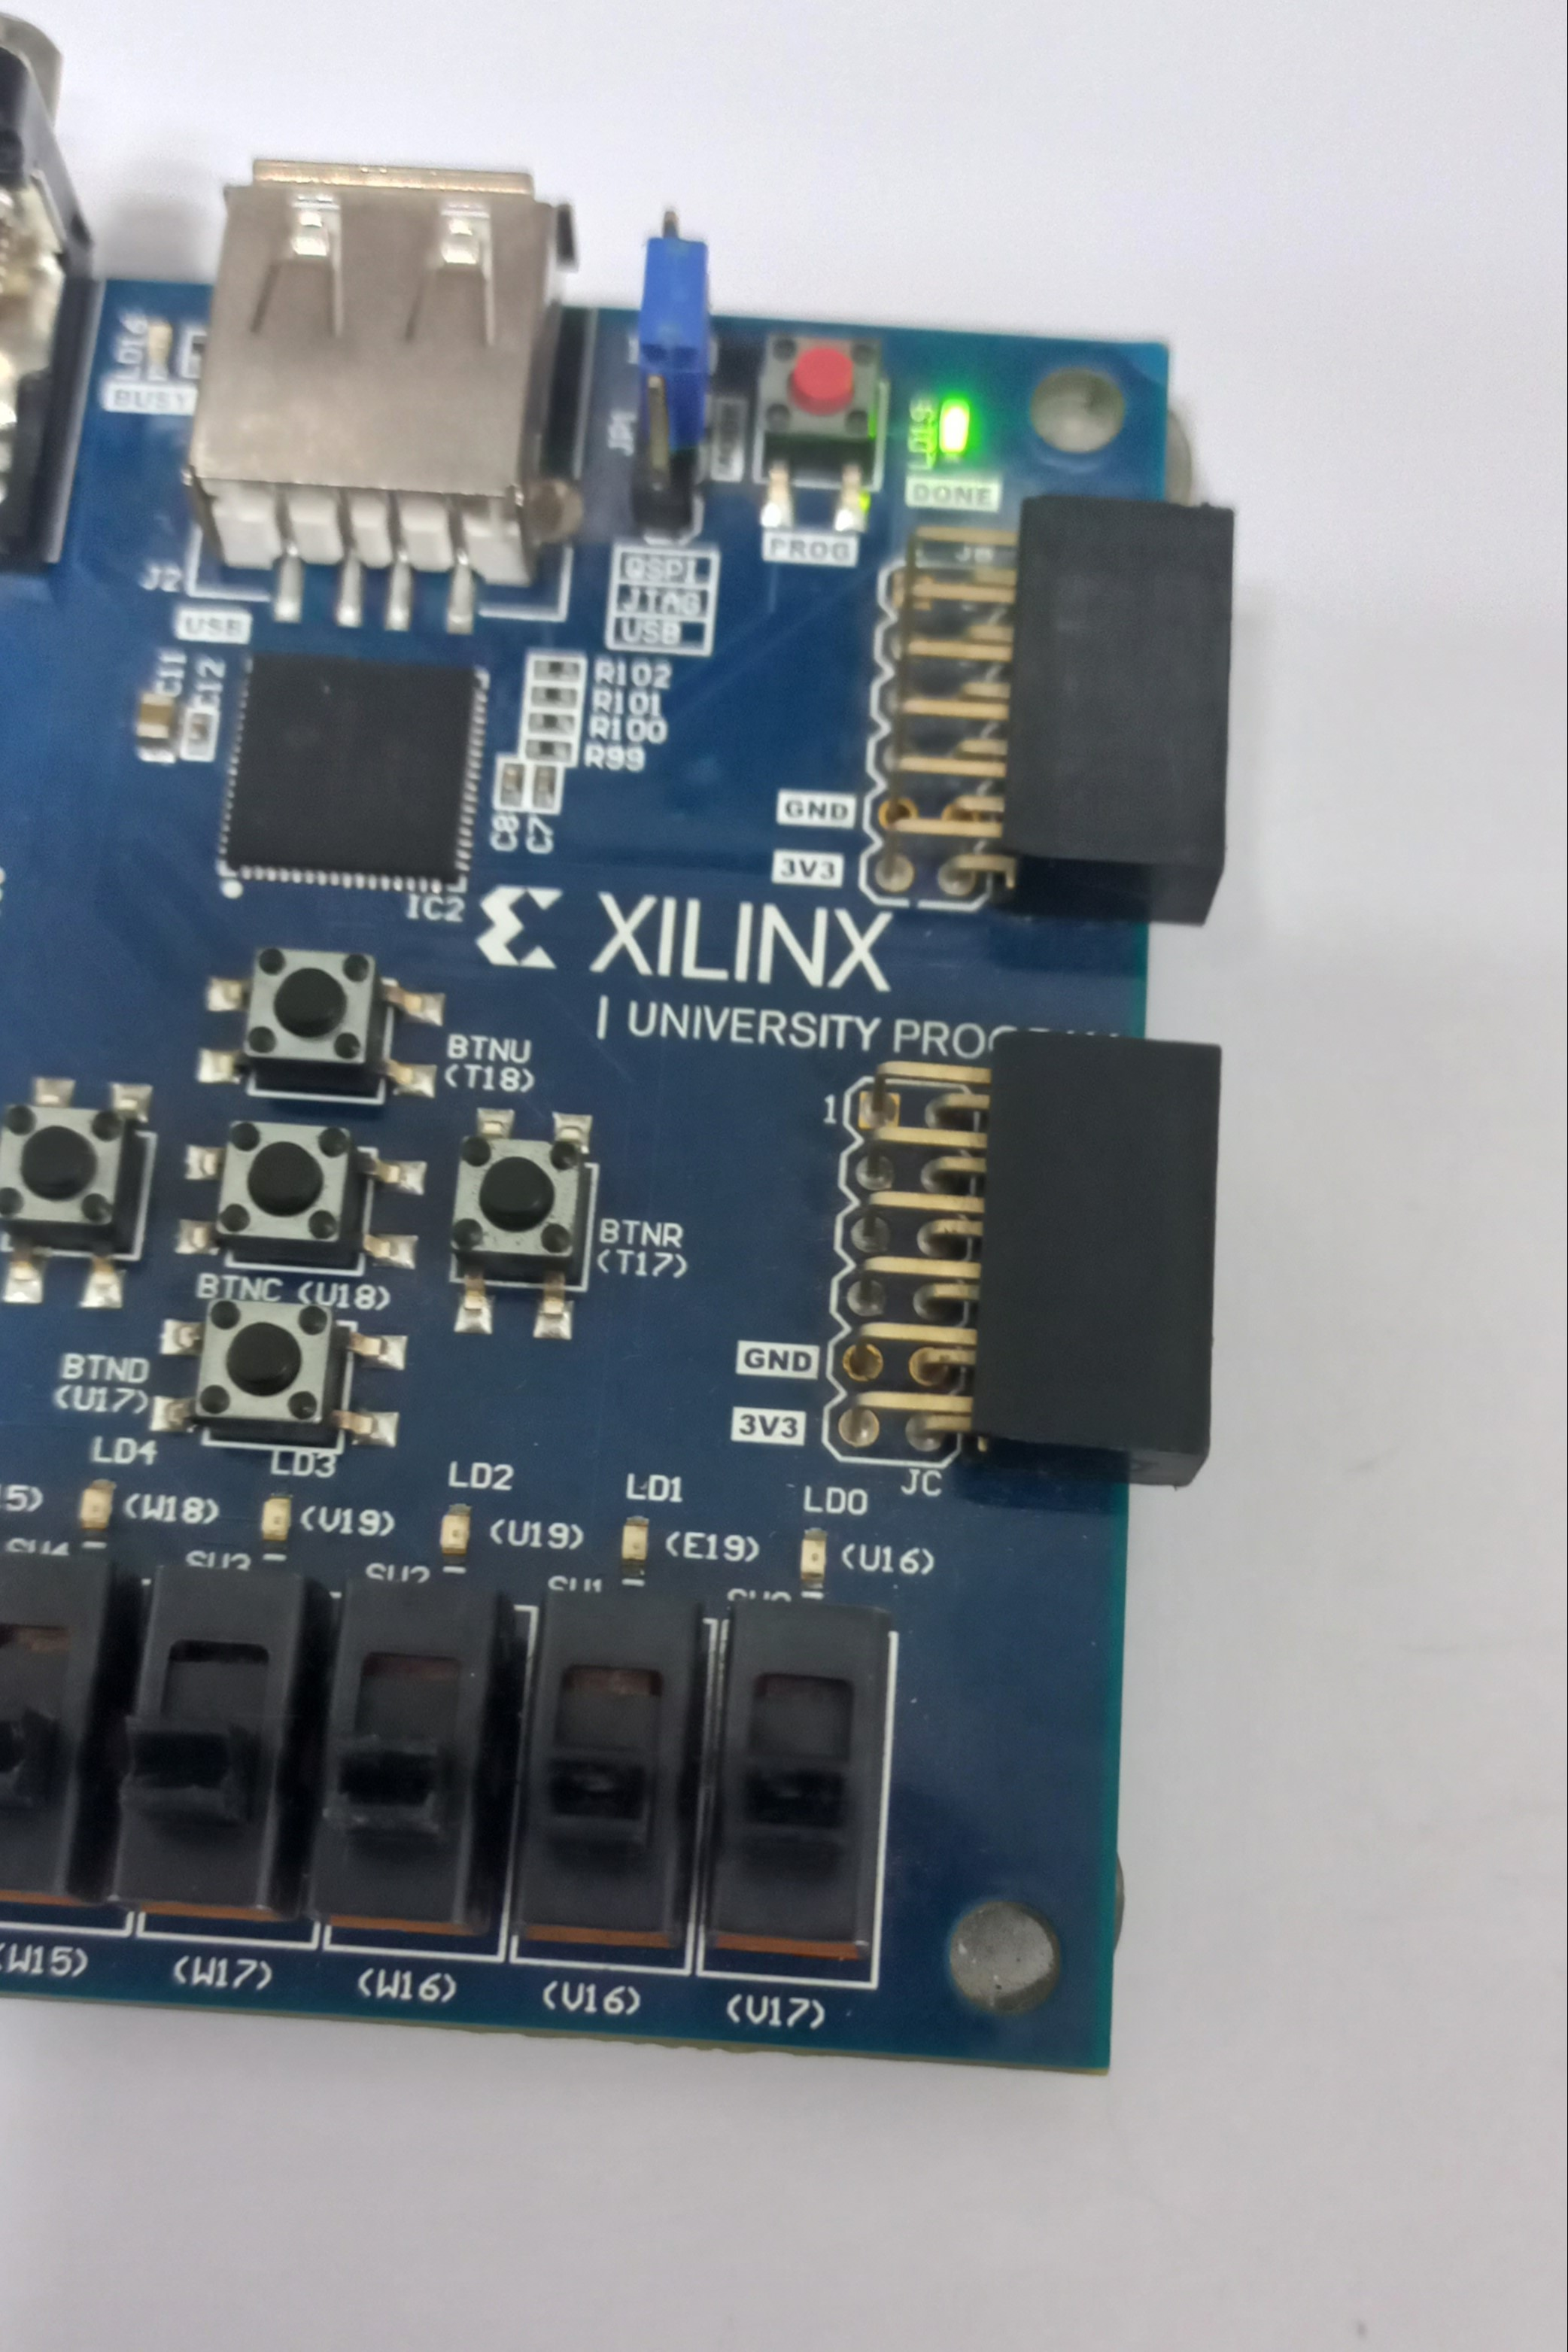
\includegraphics[width=0.3\linewidth]{simulations/demux/demux-00.jpg}
\end{figure}
\begin{figure}[!ht]
    \centering
    \caption{Demultiplexor en A=0, S=1}
    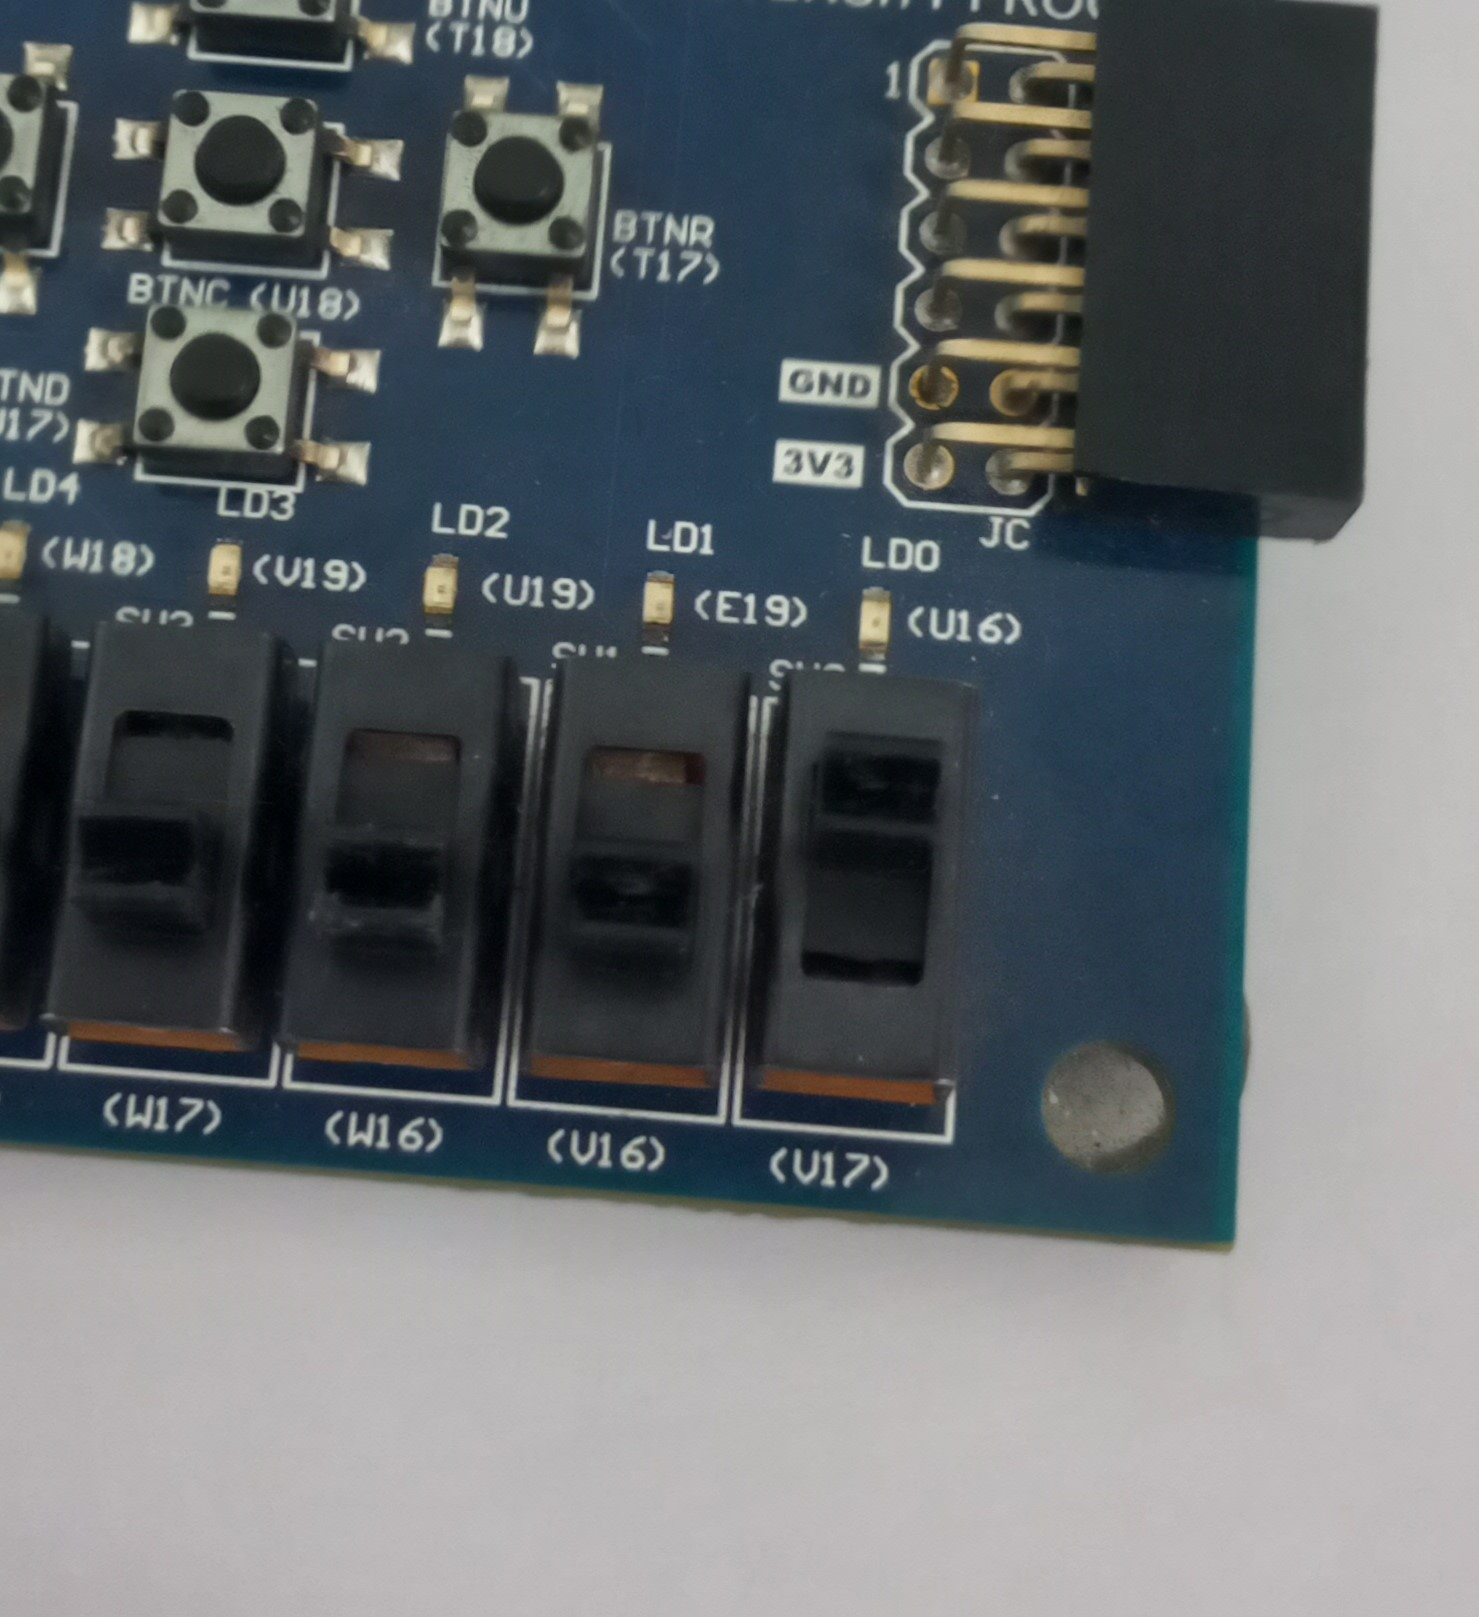
\includegraphics[width=0.3\linewidth]{simulations/demux/demux-01.jpg}
\end{figure}
\newpage

\begin{figure}[!ht]
    \centering
    \caption{Demultiplexor en A=1, S=0}
    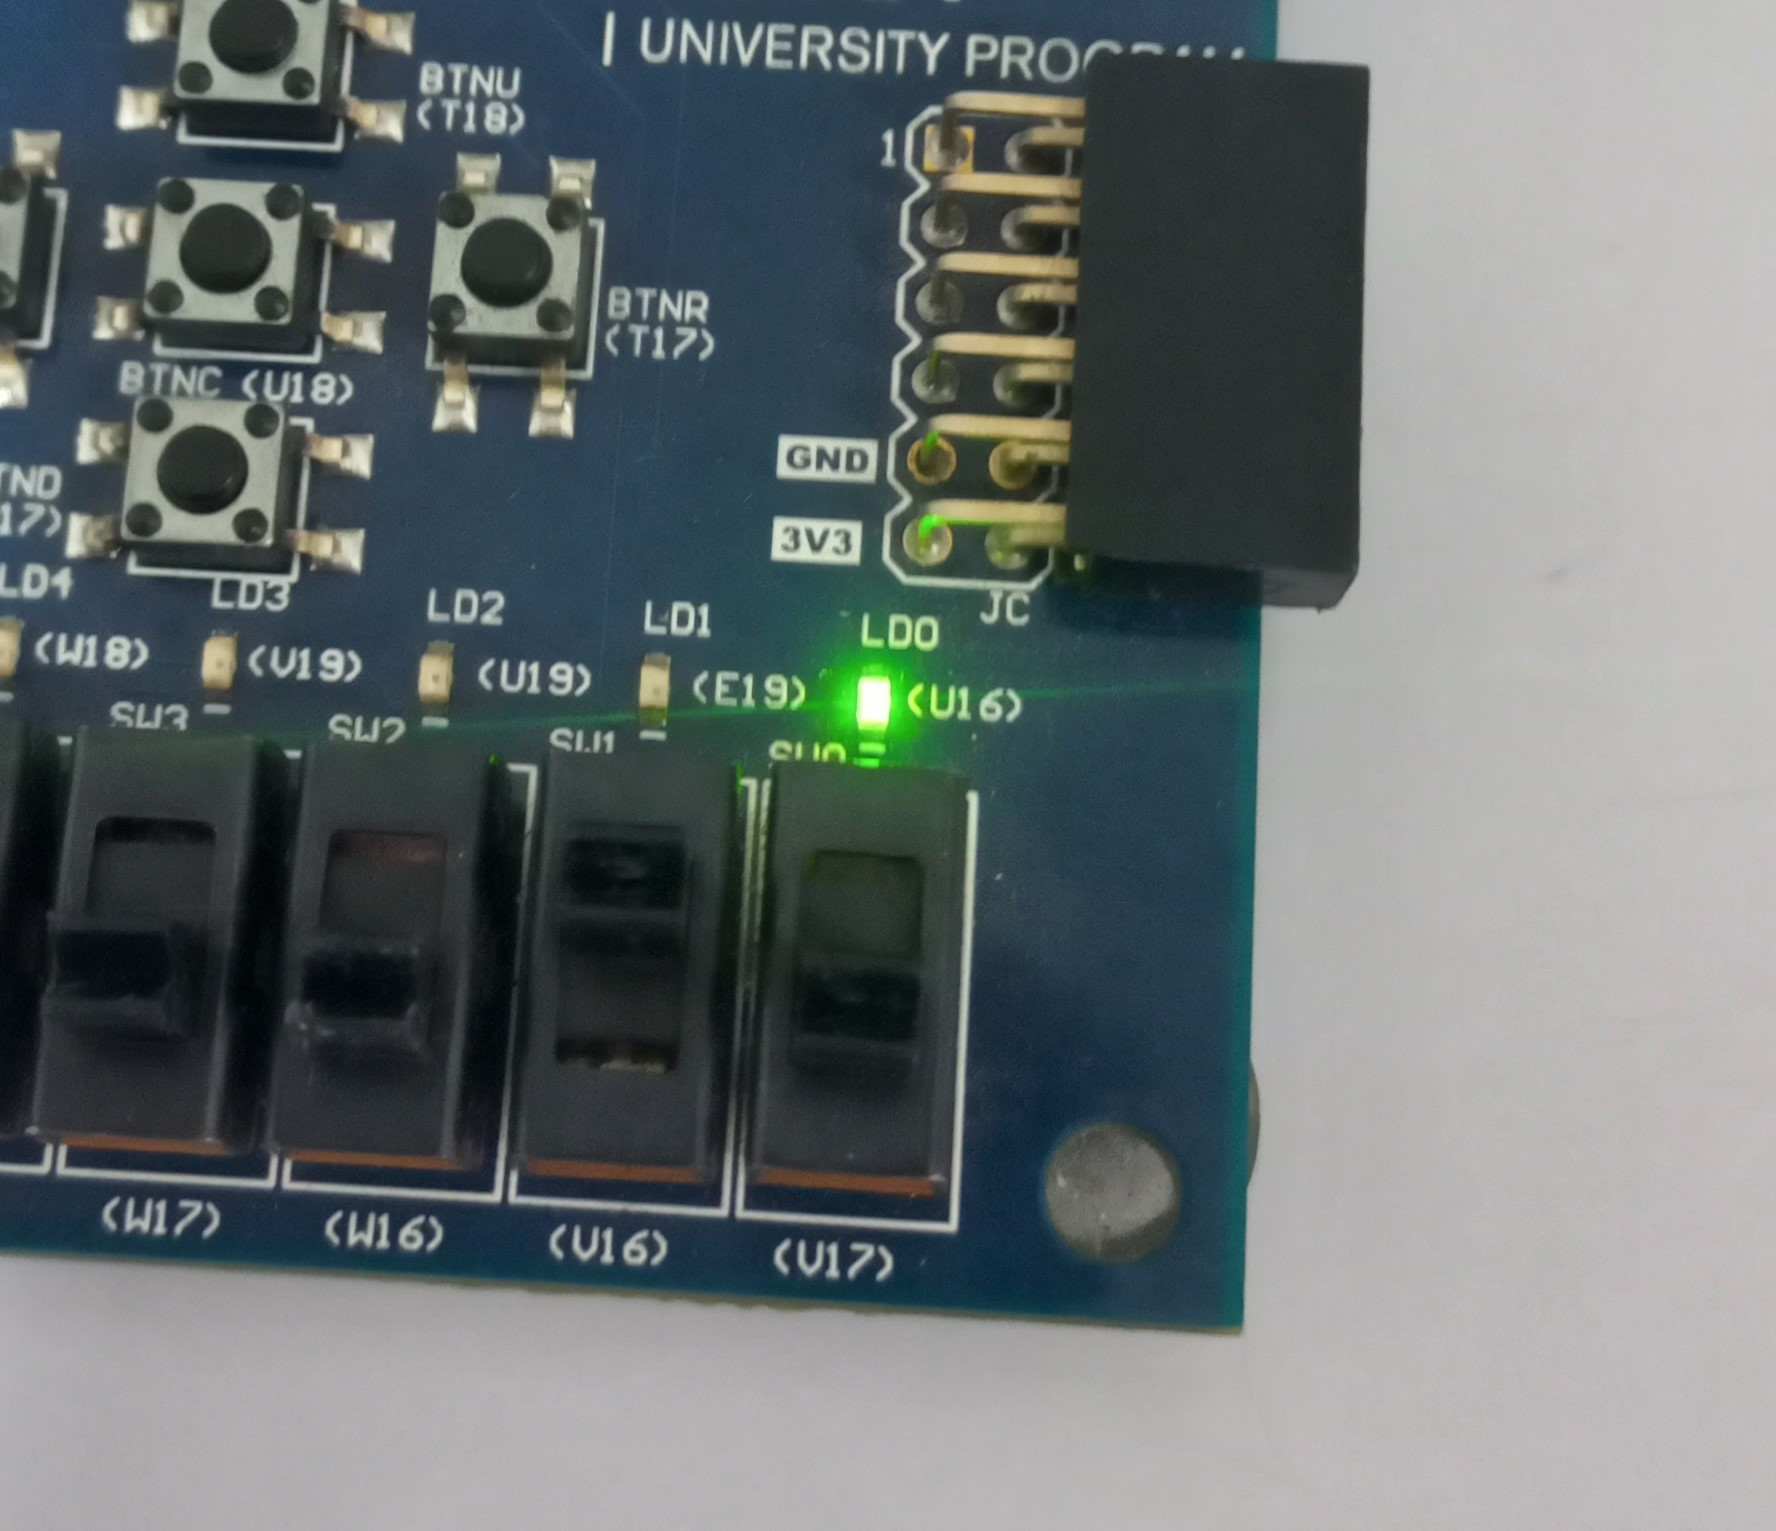
\includegraphics[width=0.5\linewidth]{simulations/demux/demux-10.jpg}
\end{figure}
\begin{figure}[!ht]
    \centering
    \caption{Demultiplexor en A=1, S=1}
    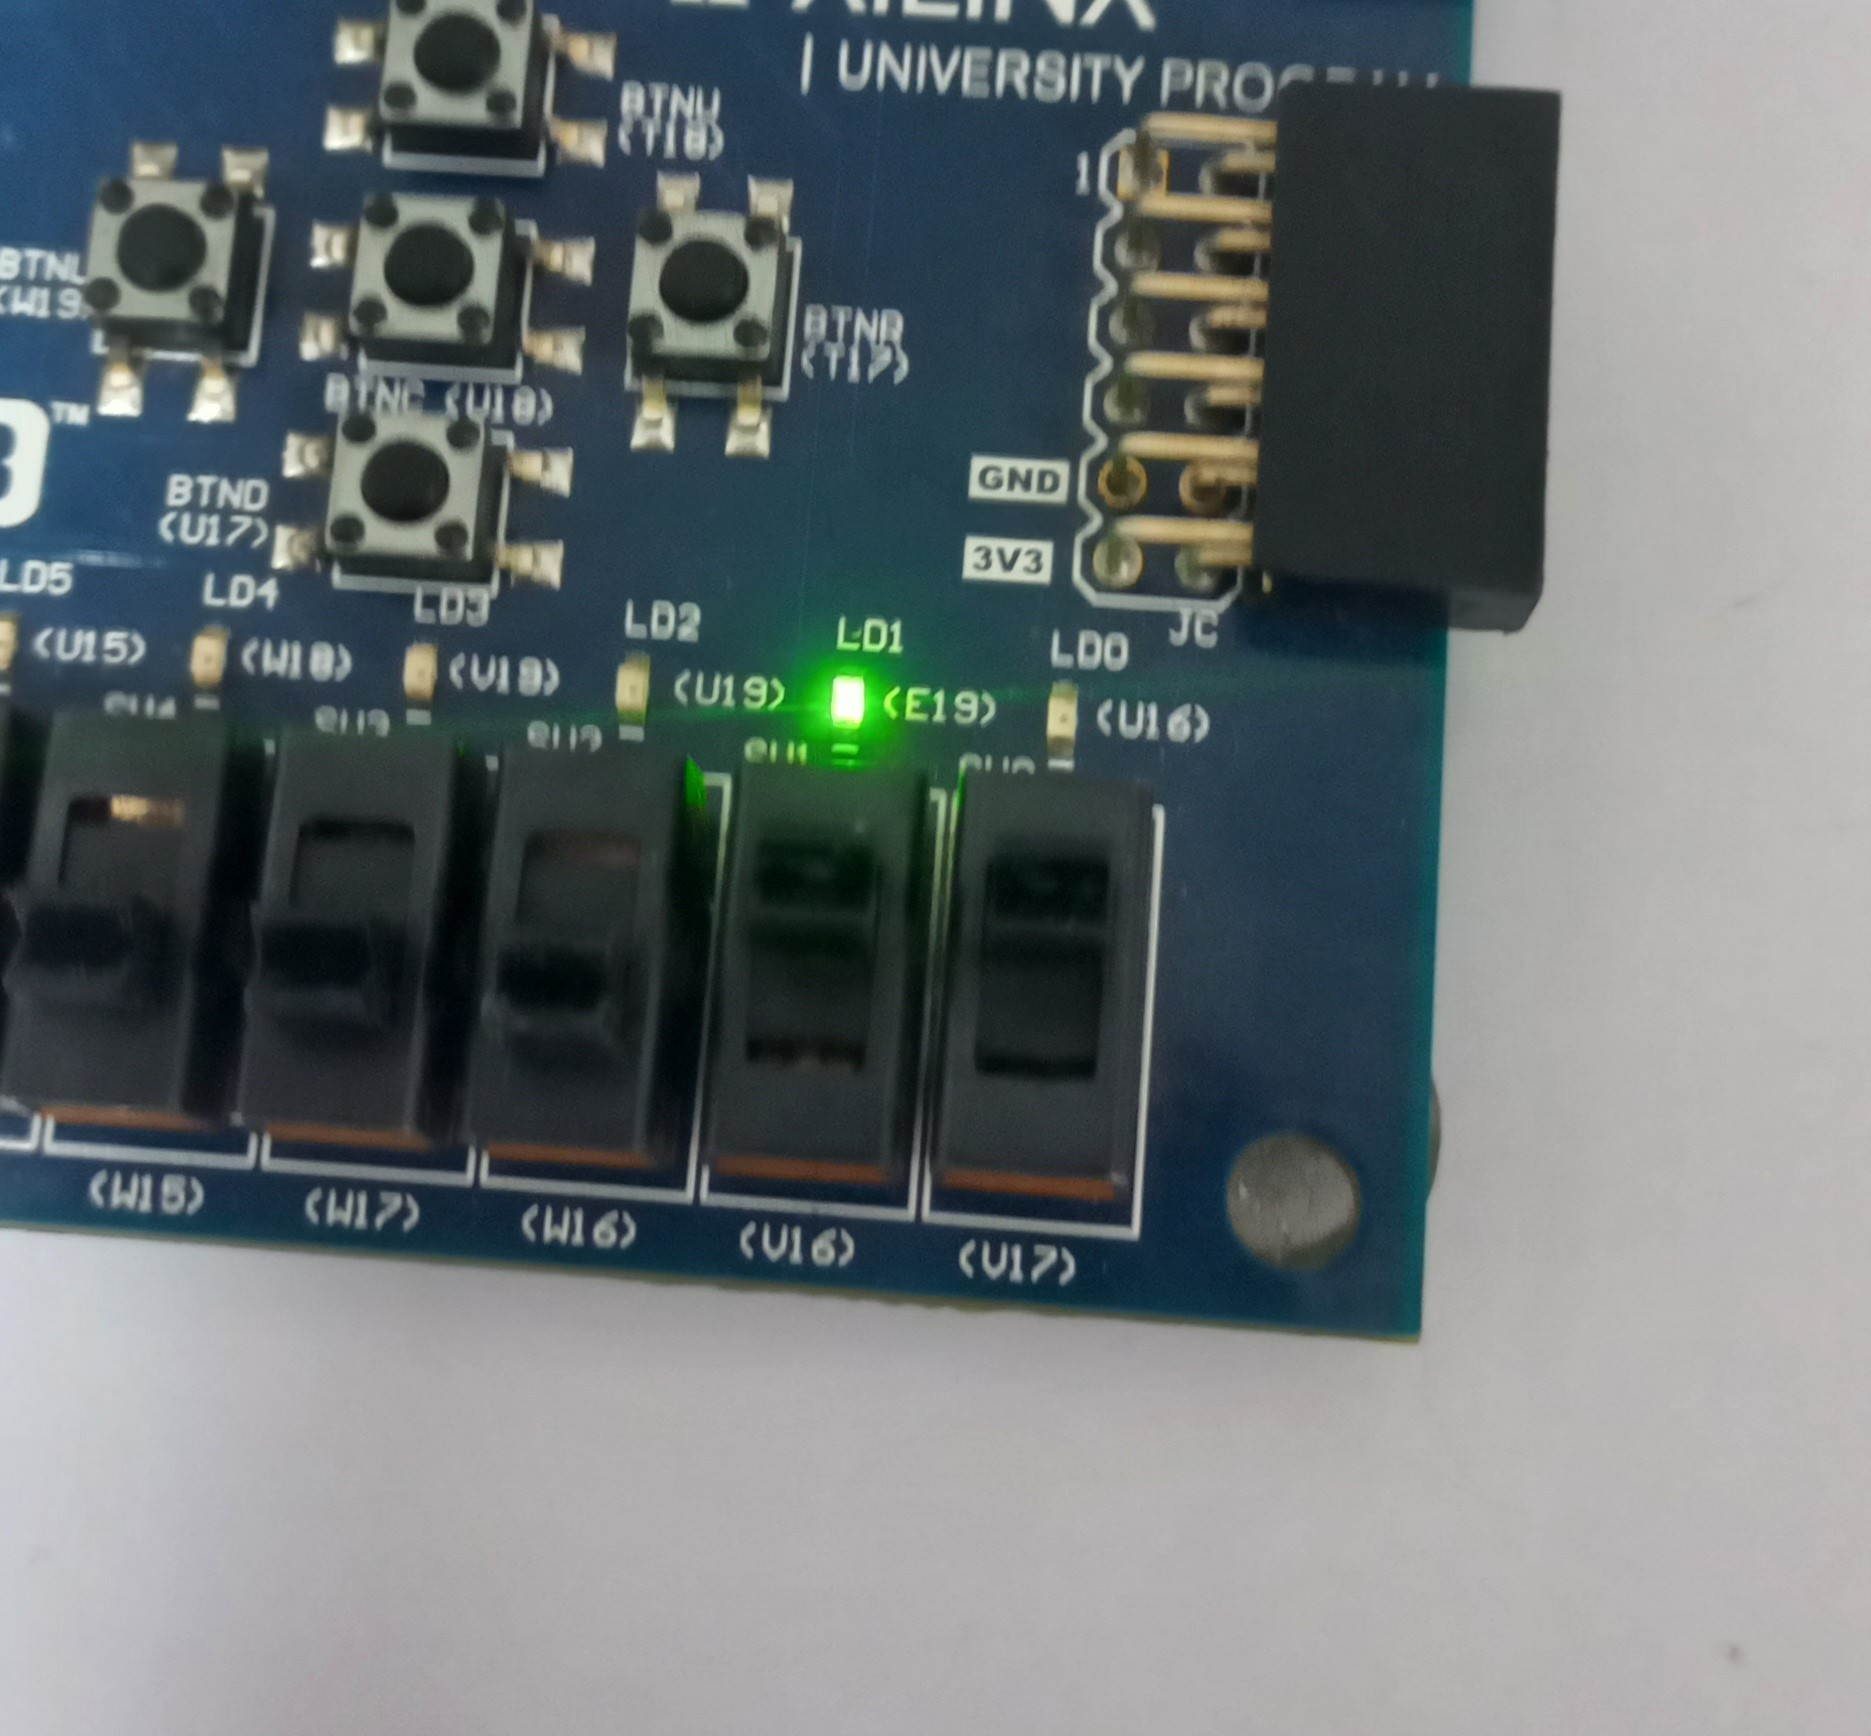
\includegraphics[width=0.5\linewidth]{simulations/demux/demux-11.jpg}
\end{figure}
\newpage

\subsection*{Códigos completos}

\lstinputlisting[language=VHDL,caption=Código Medio restador]{codigos/combinational/half.vhd}

\lstinputlisting[language=VHDL,caption=Testbench Medio restador]{codigos/tests/halftest.vhd}

\lstinputlisting[language=VHDL,caption=Código Multiplexor]{codigos/combinational/multiplexer.vhd}

\lstinputlisting[language=VHDL,caption=Testbench Multiplexor]{codigos/tests/multiplexertest.vhd}

\lstinputlisting[language=VHDL,caption=Código Comparador de magnitud]{codigos/combinational/comparador-mag.vhd}


\lstinputlisting[language=VHDL,caption= Testbench Comparador de magnitud]{codigos/tests/comparador-mag_testbench.vhd}

\lstinputlisting[language=VHDL,caption=Código demultiplexor]{codigos/combinational/demultiplexor.vhd}


\lstinputlisting[language=VHDL,caption=Testbench demultiplexor]{codigos/tests/demultiplexor_testbench.vhd}

%%%%%%% Bibliografía %%%%%%%%
\clearpage %Asegura que la bibliografía inicie en una nueva página
\bibliographystyle{bst/IEEEtran} %Estilo de bibliografía NO MODIFICAR PARA MANTENER FORMATO
\bibliography{bib/bibliografia} %Fuentes bibliográficas Se recomienda utilizar un gestor de referencias (zotero, jabref, etc..)
%%%%%%% Bibliografía %%%%%%%%
\end{document} %Termina el documento
